\chapter{A Model for Edge-Based Graph Generation} % Main chapter title
\label{ch:deep-generative-learning-graphs}
In this chapter, we introduce a novel generative model for graphs, capable of generating unattributed graphs coming from very different graph distributions. We transform graphs into sequences of ordered edges, from which we extract two sequences derived from the edge endpoints. The proposed model consists of two \glspl{rnn} to learn the probability distribution of such sequences: the first is an autoregressive network which generates a specification of the graph to produce, which is completed into a graph by the second network. We experiment extensively with the proposed model, comparing its performances with a pool of baselines, one of which is a \gls{dgm} of graphs that holds state-of-the-art performances at the generative task. The experimental framework has been designed to evaluate the proposed model on concerning both quantitative and qualitative aspects, as discussed in Section \ref{sec:evaluation-generative-graphs}. Our experiments demonstrate that, under our evaluation framework, the proposed model is able to perform at, and sometimes surpass, the state of the art in the task of generating graphs coming from very different distributions. Furthermore, we study the effect of changing the order of the edge sequence by experimenting with different node orderings. We show that the chosen node ordering strategy  is more effective for learning complex dependencies than the alternatives, and produces graphs of better quality.

\section{Methods}
In this section, we present the methodologies used to develop the model. In particular, we formally introduce the concept of ordered edge sequences, we describe the model, and we show how it is trained and how graph generation is achieved.

\subsection{Ordered Edge Sequences}
Let $\Graph{g} = \Tuple{\Nodes{g}, \Edges{g}}$ be a fully connected unattributed graph with $n$ nodes and $m$ edges. We assume $\Graph{g}$ is undirected for simplicity, without loss of generality. Let $\gamma: \Nodes{g} \shortrightarrow \Natural_{+}$ be a bijective node labelling function which assigns a unique positive integer (which we call node ID) to each node in the graph; thus, $\gamma$ defines a total order over the nodes of $\Graph{g}$. The \emph{ordered edge sequence} $\Cal{S}$ of graph $\Graph{g}$ is the sequence of pairs:
$$\OES{S}_{\Graph{g}} = ((s_1, e_1), (s_2, e_2), \ldots, (s_m, e_m)),$$
where $(\gamma^{-1}(s_i), \gamma^{-1}(e_i)) \in \Edges{g}$. Moreover, $\OES{S}_{\Graph{g}}$ is ordered lexicographically according to the IDs assigned to the nodes, \ie $(s_i,e_i) \leq (s_j,e_j)$ if and only if $s_i < s_j$, or $s_i = s_j$ and $e_i \leq e_j$. Given a generic pair $(s_i,e_i) \in \OES{S}_{\Graph{g}}$, we call $s_i \in \Natural_{+}$ its \emph{starting node} and $e_i \in \Natural_{+}$ its \emph{ending node}. Finally, let us define the \emph{starting sequence} $\Start{\OES{S}_{\Graph{g}}} = (s_1, s_2, \ldots, s_m)$, the sequence corresponding of starting nodes ordered as in $\OES{S}_{\Graph{g}}$, and analogously, the \emph{ending sequence} $\End{\OES{S}_{\Graph{g}}} = (e_1, e_2, \ldots, e_m)$, corresponding to the ending nodes ordered as in $\OES{S}_{\Graph{g}}$. For conciseness, let us omit the dependence of $\OES{S}_{\Graph{g}}$ on the graph $\Graph{g}$, and of the starting and ending sequences from $\OES{S}_{\Graph{g}}$ whenever they are clear from the context. Clearly, the choice of the labelling function $\gamma$ is critical in determining the ordered sequence of a graph. Given the graph $\Graph{g}$, we choose to implement $\gamma$ with the following algorithm:
\begin{itemize}
    \item first, select a node $v_1$ at random from its set of nodes $\Nodes{g}$, and set its node ID as $\gamma(v_1) = \SF{1}$;
    \item then, traverse the graph in breadth-first order. Let $V = (v_2, v_3, \ldots, v_{n})$ be the ordered sequence of nodes visited during the traversal, excluding $v_1$. Assign node ID $\gamma(v_i) = \SF{i},\, \forall v_i \in V,\, i=2, \ldots, n$.
\end{itemize}
Once the ordering is established, the ordered edge sequence is obtained by sorting the graph edges (now labelled by the ID of their endpoints) according to the lexicographic order. Assuming graph $\Graph{g}$ has the structure shown in Figure \ref{fig:example-graph}, and that node $v_1$ is chosen as the root node for the visit, an example of how the graph nodes are labeled by $\gamma$ is shown in Figure \ref{fig:labeled-graph}. Notice that $\gamma$ is trivially bijective, since it assigns a different integer to each node. Once the nodes are labeled, the ordered edge sequence of $\Graph{g}$ is $\OES{S} = (\OElem{1}{2},\OElem{1}{3},\OElem{1}{4},\OElem{3}{4},\OElem{3}{5})$, with $\tau_S = (\SF{1},\SF{1},\SF{1},\SF{3},\SF{3})$ and $\tau_E = (\SF{2},\SF{3},\SF{4},\SF{4},\SF{5})$. Notice that the graph can be readily reconstructed from its ordered edge sequence by first applying the inverse function $\gamma^{-1}$ to each element of its pairs to obtain $\Edges{g}$, which in turn gives $\Nodes{g}$ since we assumed that $\Graph{g}$ is fully connected.

\begin{figure*}[h!]
    \begin{subfigure}[b]{0.48\linewidth}
        \centering
        \resizebox{.8\textwidth}{!}{

\tikzset{every picture/.style={line width=0.75pt}} %set default line width to 0.75pt

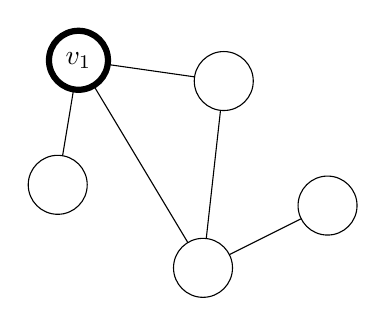
\begin{tikzpicture}[x=0.75pt,y=0.75pt,yscale=-1,xscale=1]
%uncomment if require: \path (0,169); %set diagram left start at 0, and has height of 169


% Text Node
\draw  [line width=2.25]   (45, 32) circle [x radius= 14.21, y radius= 14.21]   ;
\draw (45,32) node   [align=left] {\begin{minipage}[lt]{13.600000000000001pt}\setlength\topsep{0pt}
\begin{center}
$\displaystyle v_{1}$
\end{center}

\end{minipage}};
% Text Node
\draw    (115, 42) circle [x radius= 14.21, y radius= 14.21]   ;
\draw (115,42) node   [align=left] {\begin{minipage}[lt]{13.600000000000001pt}\setlength\topsep{0pt}
\begin{center}
$ $
\end{center}

\end{minipage}};
% Text Node
\draw    (35, 92) circle [x radius= 14.21, y radius= 14.21]   ;
\draw (35,92) node   [align=left] {\begin{minipage}[lt]{13.600000000000001pt}\setlength\topsep{0pt}
\begin{center}
$ $
\end{center}

\end{minipage}};
% Text Node
\draw    (105, 132) circle [x radius= 14.21, y radius= 14.21]   ;
\draw (105,132) node   [align=left] {\begin{minipage}[lt]{13.600000000000001pt}\setlength\topsep{0pt}
\begin{center}
\end{center}

\end{minipage}};
% Text Node
\draw    (165, 102) circle [x radius= 14.21, y radius= 14.21]   ;
\draw (165,102) node   [align=left] {\begin{minipage}[lt]{13.600000000000001pt}\setlength\topsep{0pt}
\begin{center}
$ $
\end{center}

\end{minipage}};
% Connection
\draw    (42.66,46.02) -- (37.34,77.98) ;
% Connection
\draw    (59.07,34.01) -- (100.93,39.99) ;
% Connection
\draw    (52.31,44.19) -- (97.69,119.81) ;
% Connection
\draw    (113.43,56.13) -- (106.57,117.87) ;
% Connection
\draw    (117.71,125.64) -- (152.29,108.36) ;

\end{tikzpicture}}
        \caption{}
        \label{fig:example-graph}
    \end{subfigure}
    \begin{subfigure}[b]{0.48\linewidth}
        \centering
        \resizebox{.8\textwidth}{!}{

\tikzset{every picture/.style={line width=0.75pt}} %set default line width to 0.75pt

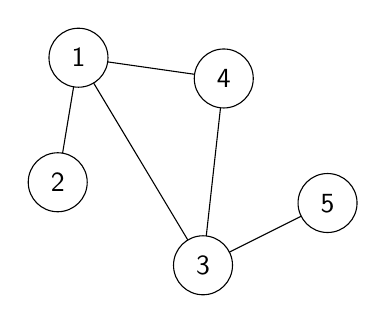
\begin{tikzpicture}[x=0.75pt,y=0.75pt,yscale=-1,xscale=1]
%uncomment if require: \path (0,181); %set diagram left start at 0, and has height of 181


% Text Node
\draw    (45, 42) circle [x radius= 14.21, y radius= 14.21]   ;
\draw (45,42) node   [align=left] {\begin{minipage}[lt]{13.600000000000001pt}\setlength\topsep{0pt}
\begin{center}
$\displaystyle \mathsf{1}$
\end{center}

\end{minipage}};
% Text Node
\draw    (115, 52) circle [x radius= 14.21, y radius= 14.21]   ;
\draw (115,52) node   [align=left] {\begin{minipage}[lt]{13.600000000000001pt}\setlength\topsep{0pt}
\begin{center}
$\displaystyle \mathsf{4}$
\end{center}

\end{minipage}};
% Text Node
\draw    (35, 102) circle [x radius= 14.21, y radius= 14.21]   ;
\draw (35,102) node   [align=left] {\begin{minipage}[lt]{13.600000000000001pt}\setlength\topsep{0pt}
\begin{center}
$\displaystyle \mathsf{2}$
\end{center}

\end{minipage}};
% Text Node
\draw    (105, 142) circle [x radius= 14.21, y radius= 14.21]   ;
\draw (105,142) node   [align=left] {\begin{minipage}[lt]{13.600000000000001pt}\setlength\topsep{0pt}
\begin{center}
$\displaystyle \mathsf{3}$
\end{center}

\end{minipage}};
% Text Node
\draw    (165, 112) circle [x radius= 14.21, y radius= 14.21]   ;
\draw (165,112) node   [align=left] {\begin{minipage}[lt]{13.600000000000001pt}\setlength\topsep{0pt}
\begin{center}
$\displaystyle \mathsf{5}$
\end{center}

\end{minipage}};
% Connection
\draw    (42.66,56.02) -- (37.34,87.98) ;
% Connection
\draw    (59.07,44.01) -- (100.93,49.99) ;
% Connection
\draw    (52.31,54.19) -- (97.69,129.81) ;
% Connection
\draw    (113.43,66.13) -- (106.57,127.87) ;
% Connection
\draw    (117.71,135.64) -- (152.29,118.36) ;

\end{tikzpicture}}
        \caption{}
        \label{fig:labeled-graph}
    \end{subfigure}
    \caption{({\scriptsize A}): an example graph, where the starting node $v_1$ of the labelling algorithm is marked with a thicker border. ({\scriptsize B}): the same graph, where nodes are labeled according to a breadth-first visit of the graph rooted at $v_1$.}
    \label{fig:labelling-example}
\end{figure*}

\subsection{Model}
Our goal is to model $p(\OES{S})$, the probability of ordered edge sequences, using a dataset $\Data = \Set{\OES{S}_{(i)}}_{i=1}^n$. Our key observation is that any ordered edge sequence $\OES{S}$ is uniquely defined by its starting and ending sequences. Therefore, instead of working on the ordered edge sequence directly, we work on their starting and ending sequences. Specifically, we model the probability of sampling $\OES{S}$ from $p(\OES{S})$ as follows:
$$p(\OES{S}) = p(\tau_S, \tau_E) = p(\tau_E \given \tau_S)\, q(\tau_S) = \prod_{i=1}^{|\OES{S}|} p(e_i \given s_i)\, \prod_{j=1}^{|\OES{S}|} q(s_j \given s_{<j}).$$
Intuitively, the generative process specified by the distribution is the following:
\begin{itemize}
    \item first, one samples $\tau_S$ from a prior probability $q(\tau_S)$, which is modeled autoregressively;
    \item once $\tau_S$ is available, it is used to condition the prediction of the ending sequence $\tau_E$.
\end{itemize}
Once both $\tau_S$ and $\tau_E$ are available, the ordered edge sequence (and thus, the corresponding graph) can be reconstructed simply pairing their elements. Here, we make an important remark. Notice that the probability of $q(\tau_S)$ is modeled autoregressively, while the conditional $p(\tau_E \given \tau_S)$ is not. This means that to generate a sequence, the only stochastic part in the model relates to $q(\tau_S)$, while predicting $\tau_E$ is deterministic once $\tau_S$ is known. One possible interpretation of $q(\tau_S)$ is that it acts as a \quotes{soft prior} of the structure of the graph: in fact, it specifies a subset of relevant nodes for the generation and their degree, expressed as the number of times they appear in the starting sequence. The conditional $p(\tau_E \given \tau_S)$ uses this information to \quotes{complete} the graph based on the information provided by the prior.

\subsection{Training}
The model specified above is implemented as two \glspl{rnn} in cascade, which we refer to as $q_{\EncParam}$ and $p_{\DecParam}$ respectively. The two sequences (starting and ending) are first encoded as sequences of $(k+2)$-dimensional one-hot vectors, where $k$ is the largest node ID assigned by $\gamma$ to any node in the dataset, and $+2$ is added for the start of sequence and end of sequence tokens. We indicate the one-hot encoded starting sequence with the notation $\Vector{s} = (\Elem{s}{1}, \ldots, \Elem{s}{|\tau_S|}, \EOS)$, where $\Elem{s}{i} \in \Real^{k+2}$, and analogously, we use $\Vector{e} = (\Elem{e}{1}, \ldots, \Elem{e}{|\tau_E|})$ for the one-hot encoded ending sequence, with $\Elem{e}{i} \in \Real^{k+2}$. Notice that an end of sequence token is added to $\Vector{s}$: when it is predicted, the autoregressive process that yields $\Vector{s}$ is interrupted. Our dataset has thus the following form: $\Data = \Set{(\Vector{s}_{(i)}, \Vector{e}_{(i)})}_{i=1}^n$. Focusing on a single training pair $(\Vector{s}, \Vector{e})$, we explain the feed-forward phase of the network. Firstly, the sequence $\Vector{s}$ is processed by $q_{\EncParam}$. Given an element $\Elem{s}{i} \in \Vector{s}$, the per-element output of $q_{\EncParam}$ is obtained as follows:
\begin{align*}
    \Elem{h}{i} &= \Op{GRU}_{\EncParam}(\Matrix{E}^{\Transpose}\Elem{s}{i-1}, \Elem{h}{i-1})\\
    \Elem{o}{i} &= \softmax(\Matrix{V}_{\EncParam}\Elem{h}{i} + \Vector{b}_{\EncParam}).
\end{align*}
In the formula above, $\Matrix{E} \in \Real^{h \times (k+2)}$ is an \emph{embedding matrix} whose entries are learnable, and the dot product selects the column of $\Vector{E}$ corresponding to the embedding of the node ID assigned to $\Elem{s}{i}$. Furthermore, $\Elem{h}{i} \in \Real^h$ is a hidden state, $\Op{GRU}_{\EncParam}$ is a multi-layer GRU network, $\Matrix{V}_{\EncParam} \in \Real^{(k+2)\times h}$ and $\Vector{b}_{\EncParam} \in \Real^{k+2}$ are the weights of the softmax output layer, and $\Elem{o}{i}$ is an output distribution over all the possible node IDs. The process is initialized by setting $\Elem{s}{0} = \SOS$ and $\Elem{h}{0} = \Zeros$. We use teacher forcing, meaning that, at each step, the input of the network is the ground truth value taken from $\Vector{s}$, rather than the output predicted by the network. Lastly, the output $\Elem{o}{i}$ is compared to the ground truth value $\Elem{s}{i}$ using the \gls{ce} loss function. For the whole starting sequence, the computed loss is the following:
$$\Loss(\EncParam, \Vector{s}) = \frac{1}{|\Vector{s}|+1} \sum_{i=1}^{|\Vector{s}|+1} q_{\EncParam}(\Elem{s}{i} \given \Elem{s}{<i}) = \frac{1}{|\Vector{s}|+1} \sum_{i=1}^{|\Vector{s}|+1} \mathrm{CE}(\Elem{s}{i}, \Elem{o}{i}).$$
After the starting sequence $\Vector{s}$ has been processed by $q_{\EncParam}$, the control flow passes onto $p_{\DecParam}$. The function computed by $p_{\DecParam}$ is similar to the one implemented by the first \gls{rnn}. Specifically, it is the following:
\begin{align*}
    \Elem{h'}{i} &= \Op{GRU}_{\DecParam}(\Matrix{E}^{\Transpose}\Elem{s}{i}, \Elem{h'}{i-1})\\
    \Elem{o'}{i} &= \softmax(\Matrix{V}_{\DecParam}\Elem{h'}{i} + \Vector{b'}_{\DecParam}),
\end{align*}
where $\Elem{h'}{0} = \Elem{h}{|\tau_S|}$, \ie the second network is initialized with the last hidden state of the first. Moreover, $\Elem{h'}{i} \in \Real^h$ is a hidden state, $\Op{GRU}_{\DecParam}$ is a multi-layer GRU network, $\Matrix{V}_{\DecParam} \in \Real^{(k+2) \times h}$ and $\Vector{b'}_{\Param} \in \Real^{k+2}$ are the weights of the softmax output layer, $\Elem{o}{i}$ is an output distribution over all the possible node IDs, and $\Matrix{E}$ is the same embedding matrix used by $q_{\EncParam}$.  Lastly, the output $\Elem{o'}{i}$ is compared to the ground truth value $\Elem{e}{i}$ using the \gls{ce} loss function, similarly as before. For the whole ending sequence, the computed loss is the following:
$$\Loss(\DecParam, (\Vector{s}, \Vector{e})) = \frac{1}{|\Vector{e}|} \sum_{i=1}^{|\Vector{e}|} - \log p_{\DecParam}(\Elem{e}{i} \given \Elem{s}{i}) = \frac{1}{|\Vector{e}|} \sum_{i=1}^{|\Vector{e}|} \mathrm{CE}(\Elem{e}{i}, \Elem{o'}{i}).$$
The whole network is trained with \gls{mle} by minimizing the following objective function:
$$\argmin_{\Param} \frac{1}{n} \sum_{(\Vector{s},\Vector{e}) \in \Data} \Loss(\EncParam, \Vector{s}) + \Loss(\DecParam, (\Vector{s}, \Vector{e})),$$
where $\Param = (\DecParam, \EncParam)$. Figure \ref{fig:model-training} shows the architecture during training.

\begin{figure*}[h!]
    \centering
    \resizebox{.8\textwidth}{!}{

\tikzset{every picture/.style={line width=0.75pt}} %set default line width to 0.75pt

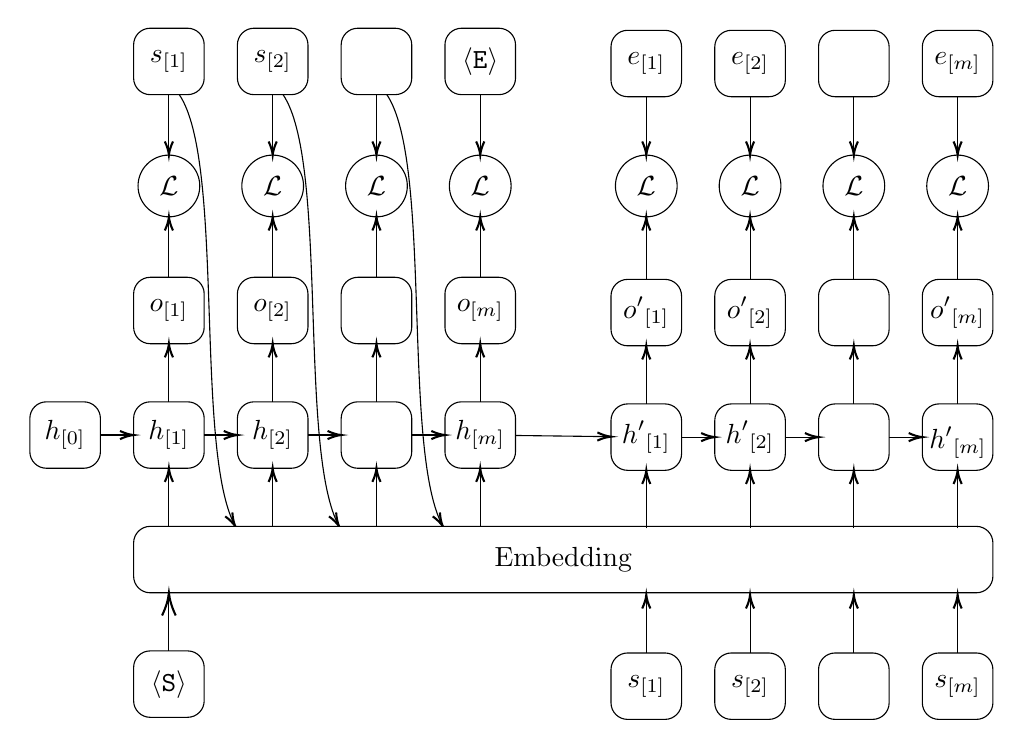
\begin{tikzpicture}[x=0.75pt,y=0.75pt,yscale=-1,xscale=1]
%uncomment if require: \path (0,400); %set diagram left start at 0, and has height of 400

%Curve Lines [id:da14509372882198068]
\draw    (100,62) .. controls (121.77,94.16) and (107.54,229.5) .. (126.13,268.3) ;
\draw [shift={(127,270)}, rotate = 241.3] [color={rgb, 255:red, 0; green, 0; blue, 0 }  ][line width=0.75]    (6.56,-1.97) .. controls (4.17,-0.84) and (1.99,-0.18) .. (0,0) .. controls (1.99,0.18) and (4.17,0.84) .. (6.56,1.97)   ;
%Curve Lines [id:da32690755901594937]
\draw    (150,62) .. controls (171.77,94.16) and (157.54,229.5) .. (176.13,268.3) ;
\draw [shift={(177,270)}, rotate = 241.3] [color={rgb, 255:red, 0; green, 0; blue, 0 }  ][line width=0.75]    (6.56,-1.97) .. controls (4.17,-0.84) and (1.99,-0.18) .. (0,0) .. controls (1.99,0.18) and (4.17,0.84) .. (6.56,1.97)   ;
%Curve Lines [id:da8801757764435838]
\draw    (200,62) .. controls (221.77,94.16) and (207.54,229.5) .. (226.13,268.3) ;
\draw [shift={(227,270)}, rotate = 241.3] [color={rgb, 255:red, 0; green, 0; blue, 0 }  ][line width=0.75]    (6.56,-1.97) .. controls (4.17,-0.84) and (1.99,-0.18) .. (0,0) .. controls (1.99,0.18) and (4.17,0.84) .. (6.56,1.97)   ;

% Text Node
\draw  [fill={rgb, 255:red, 255; green, 255; blue, 255 }  ,fill opacity=1 ]  (78,278) .. controls (78,273.58) and (81.58,270) .. (86,270) -- (484,270) .. controls (488.42,270) and (492,273.58) .. (492,278) -- (492,294) .. controls (492,298.42) and (488.42,302) .. (484,302) -- (86,302) .. controls (81.58,302) and (78,298.42) .. (78,294) -- cycle  ;
\draw (285,286) node   [align=left] {\begin{minipage}[lt]{278.8pt}\setlength\topsep{0pt}
\begin{center}
Embedding
\end{center}

\end{minipage}};
% Text Node
\draw (95,286) node   [align=left] {\begin{minipage}[lt]{20.400000000000002pt}\setlength\topsep{0pt}
\begin{center}
\end{center}

\end{minipage}};
% Text Node
\draw (145,286) node   [align=left] {\begin{minipage}[lt]{20.400000000000002pt}\setlength\topsep{0pt}
\begin{center}
\end{center}

\end{minipage}};
% Text Node
\draw (195,286) node   [align=left] {\begin{minipage}[lt]{20.400000000000002pt}\setlength\topsep{0pt}
\begin{center}
\end{center}

\end{minipage}};
% Text Node
\draw (245,286) node   [align=left] {\begin{minipage}[lt]{20.400000000000002pt}\setlength\topsep{0pt}
\begin{center}
\end{center}

\end{minipage}};
% Text Node
\draw    (78,218) .. controls (78,213.58) and (81.58,210) .. (86,210) -- (104,210) .. controls (108.42,210) and (112,213.58) .. (112,218) -- (112,234) .. controls (112,238.42) and (108.42,242) .. (104,242) -- (86,242) .. controls (81.58,242) and (78,238.42) .. (78,234) -- cycle  ;
\draw (95,226) node   [align=left] {\begin{minipage}[lt]{20.400000000000002pt}\setlength\topsep{0pt}
\begin{center}
$\displaystyle \boldsymbol{h}_{[ 1]}$
\end{center}

\end{minipage}};
% Text Node
\draw    (128,218) .. controls (128,213.58) and (131.58,210) .. (136,210) -- (154,210) .. controls (158.42,210) and (162,213.58) .. (162,218) -- (162,234) .. controls (162,238.42) and (158.42,242) .. (154,242) -- (136,242) .. controls (131.58,242) and (128,238.42) .. (128,234) -- cycle  ;
\draw (145,226) node   [align=left] {\begin{minipage}[lt]{20.400000000000002pt}\setlength\topsep{0pt}
\begin{center}
$\displaystyle \boldsymbol{h}_{[ 2]}$
\end{center}

\end{minipage}};
% Text Node
\draw    (178,218) .. controls (178,213.58) and (181.58,210) .. (186,210) -- (204,210) .. controls (208.42,210) and (212,213.58) .. (212,218) -- (212,234) .. controls (212,238.42) and (208.42,242) .. (204,242) -- (186,242) .. controls (181.58,242) and (178,238.42) .. (178,234) -- cycle  ;
\draw (195,226) node   [align=left] {\begin{minipage}[lt]{20.400000000000002pt}\setlength\topsep{0pt}
\begin{center}
$\displaystyle \dotsc $
\end{center}

\end{minipage}};
% Text Node
\draw    (228,218) .. controls (228,213.58) and (231.58,210) .. (236,210) -- (254,210) .. controls (258.42,210) and (262,213.58) .. (262,218) -- (262,234) .. controls (262,238.42) and (258.42,242) .. (254,242) -- (236,242) .. controls (231.58,242) and (228,238.42) .. (228,234) -- cycle  ;
\draw (245,226) node   [align=left] {\begin{minipage}[lt]{20.400000000000002pt}\setlength\topsep{0pt}
\begin{center}
$\displaystyle \boldsymbol{h}_{[ m]}$
\end{center}

\end{minipage}};
% Text Node
\draw    (78,158) .. controls (78,153.58) and (81.58,150) .. (86,150) -- (104,150) .. controls (108.42,150) and (112,153.58) .. (112,158) -- (112,174) .. controls (112,178.42) and (108.42,182) .. (104,182) -- (86,182) .. controls (81.58,182) and (78,178.42) .. (78,174) -- cycle  ;
\draw (95,166) node   [align=left] {\begin{minipage}[lt]{20.400000000000002pt}\setlength\topsep{0pt}
\begin{center}
$\displaystyle \boldsymbol{o}_{[ 1]}$
\end{center}

\end{minipage}};
% Text Node
\draw    (128,158) .. controls (128,153.58) and (131.58,150) .. (136,150) -- (154,150) .. controls (158.42,150) and (162,153.58) .. (162,158) -- (162,174) .. controls (162,178.42) and (158.42,182) .. (154,182) -- (136,182) .. controls (131.58,182) and (128,178.42) .. (128,174) -- cycle  ;
\draw (145,166) node   [align=left] {\begin{minipage}[lt]{20.400000000000002pt}\setlength\topsep{0pt}
\begin{center}
$\displaystyle \boldsymbol{o}_{[ 2]}$
\end{center}

\end{minipage}};
% Text Node
\draw    (178,158) .. controls (178,153.58) and (181.58,150) .. (186,150) -- (204,150) .. controls (208.42,150) and (212,153.58) .. (212,158) -- (212,174) .. controls (212,178.42) and (208.42,182) .. (204,182) -- (186,182) .. controls (181.58,182) and (178,178.42) .. (178,174) -- cycle  ;
\draw (195,166) node   [align=left] {\begin{minipage}[lt]{20.400000000000002pt}\setlength\topsep{0pt}
\begin{center}
$\displaystyle \dotsc $
\end{center}

\end{minipage}};
% Text Node
\draw    (228,158) .. controls (228,153.58) and (231.58,150) .. (236,150) -- (254,150) .. controls (258.42,150) and (262,153.58) .. (262,158) -- (262,174) .. controls (262,178.42) and (258.42,182) .. (254,182) -- (236,182) .. controls (231.58,182) and (228,178.42) .. (228,174) -- cycle  ;
\draw (245,166) node   [align=left] {\begin{minipage}[lt]{20.400000000000002pt}\setlength\topsep{0pt}
\begin{center}
$\displaystyle \boldsymbol{o}_{[ m]}$
\end{center}

\end{minipage}};
% Text Node
\draw    (308,339) .. controls (308,334.58) and (311.58,331) .. (316,331) -- (334,331) .. controls (338.42,331) and (342,334.58) .. (342,339) -- (342,355) .. controls (342,359.42) and (338.42,363) .. (334,363) -- (316,363) .. controls (311.58,363) and (308,359.42) .. (308,355) -- cycle  ;
\draw (325,347) node   [align=left] {\begin{minipage}[lt]{20.400000000000002pt}\setlength\topsep{0pt}
\begin{center}
$\displaystyle \boldsymbol{s}_{[ 1]}$
\end{center}

\end{minipage}};
% Text Node
\draw (325,287) node   [align=left] {\begin{minipage}[lt]{20.400000000000002pt}\setlength\topsep{0pt}
\begin{center}
\end{center}

\end{minipage}};
% Text Node
\draw    (358,339) .. controls (358,334.58) and (361.58,331) .. (366,331) -- (384,331) .. controls (388.42,331) and (392,334.58) .. (392,339) -- (392,355) .. controls (392,359.42) and (388.42,363) .. (384,363) -- (366,363) .. controls (361.58,363) and (358,359.42) .. (358,355) -- cycle  ;
\draw (375,347) node   [align=left] {\begin{minipage}[lt]{20.400000000000002pt}\setlength\topsep{0pt}
\begin{center}
$\displaystyle \boldsymbol{s}_{[ 2]}$
\end{center}

\end{minipage}};
% Text Node
\draw    (408,339) .. controls (408,334.58) and (411.58,331) .. (416,331) -- (434,331) .. controls (438.42,331) and (442,334.58) .. (442,339) -- (442,355) .. controls (442,359.42) and (438.42,363) .. (434,363) -- (416,363) .. controls (411.58,363) and (408,359.42) .. (408,355) -- cycle  ;
\draw (425,347) node   [align=left] {\begin{minipage}[lt]{20.400000000000002pt}\setlength\topsep{0pt}
\begin{center}
$\displaystyle \dotsc $
\end{center}

\end{minipage}};
% Text Node
\draw    (458,339) .. controls (458,334.58) and (461.58,331) .. (466,331) -- (484,331) .. controls (488.42,331) and (492,334.58) .. (492,339) -- (492,355) .. controls (492,359.42) and (488.42,363) .. (484,363) -- (466,363) .. controls (461.58,363) and (458,359.42) .. (458,355) -- cycle  ;
\draw (475,347) node   [align=left] {\begin{minipage}[lt]{20.400000000000002pt}\setlength\topsep{0pt}
\begin{center}
$\displaystyle \boldsymbol{s}_{[ m]}$
\end{center}

\end{minipage}};
% Text Node
\draw (375,287) node   [align=left] {\begin{minipage}[lt]{20.400000000000002pt}\setlength\topsep{0pt}
\begin{center}
\end{center}

\end{minipage}};
% Text Node
\draw (425,287) node   [align=left] {\begin{minipage}[lt]{20.400000000000002pt}\setlength\topsep{0pt}
\begin{center}
\end{center}

\end{minipage}};
% Text Node
\draw (475,287) node   [align=left] {\begin{minipage}[lt]{20.400000000000002pt}\setlength\topsep{0pt}
\begin{center}
\end{center}

\end{minipage}};
% Text Node
\draw    (308,219) .. controls (308,214.58) and (311.58,211) .. (316,211) -- (334,211) .. controls (338.42,211) and (342,214.58) .. (342,219) -- (342,235) .. controls (342,239.42) and (338.42,243) .. (334,243) -- (316,243) .. controls (311.58,243) and (308,239.42) .. (308,235) -- cycle  ;
\draw (325,227) node   [align=left] {\begin{minipage}[lt]{20.400000000000002pt}\setlength\topsep{0pt}
\begin{center}
$\displaystyle \boldsymbol{h'}_{[ 1]}$
\end{center}

\end{minipage}};
% Text Node
\draw    (358,219) .. controls (358,214.58) and (361.58,211) .. (366,211) -- (384,211) .. controls (388.42,211) and (392,214.58) .. (392,219) -- (392,235) .. controls (392,239.42) and (388.42,243) .. (384,243) -- (366,243) .. controls (361.58,243) and (358,239.42) .. (358,235) -- cycle  ;
\draw (375,227) node   [align=left] {\begin{minipage}[lt]{20.400000000000002pt}\setlength\topsep{0pt}
\begin{center}
$\displaystyle \boldsymbol{h'}_{[ 2]}$
\end{center}

\end{minipage}};
% Text Node
\draw    (408,219) .. controls (408,214.58) and (411.58,211) .. (416,211) -- (434,211) .. controls (438.42,211) and (442,214.58) .. (442,219) -- (442,235) .. controls (442,239.42) and (438.42,243) .. (434,243) -- (416,243) .. controls (411.58,243) and (408,239.42) .. (408,235) -- cycle  ;
\draw (425,227) node   [align=left] {\begin{minipage}[lt]{20.400000000000002pt}\setlength\topsep{0pt}
\begin{center}
$\displaystyle \dotsc $
\end{center}

\end{minipage}};
% Text Node
\draw    (458,219) .. controls (458,214.58) and (461.58,211) .. (466,211) -- (484,211) .. controls (488.42,211) and (492,214.58) .. (492,219) -- (492,235) .. controls (492,239.42) and (488.42,243) .. (484,243) -- (466,243) .. controls (461.58,243) and (458,239.42) .. (458,235) -- cycle  ;
\draw (475,227) node   [align=left] {\begin{minipage}[lt]{20.400000000000002pt}\setlength\topsep{0pt}
\begin{center}
$\displaystyle \boldsymbol{h'}_{[ m]}$
\end{center}

\end{minipage}};
% Text Node
\draw    (308,159) .. controls (308,154.58) and (311.58,151) .. (316,151) -- (334,151) .. controls (338.42,151) and (342,154.58) .. (342,159) -- (342,175) .. controls (342,179.42) and (338.42,183) .. (334,183) -- (316,183) .. controls (311.58,183) and (308,179.42) .. (308,175) -- cycle  ;
\draw (325,167) node   [align=left] {\begin{minipage}[lt]{20.400000000000002pt}\setlength\topsep{0pt}
\begin{center}
$\displaystyle \boldsymbol{o'}_{[ 1]}$
\end{center}

\end{minipage}};
% Text Node
\draw    (358,159) .. controls (358,154.58) and (361.58,151) .. (366,151) -- (384,151) .. controls (388.42,151) and (392,154.58) .. (392,159) -- (392,175) .. controls (392,179.42) and (388.42,183) .. (384,183) -- (366,183) .. controls (361.58,183) and (358,179.42) .. (358,175) -- cycle  ;
\draw (375,167) node   [align=left] {\begin{minipage}[lt]{20.400000000000002pt}\setlength\topsep{0pt}
\begin{center}
$\displaystyle \boldsymbol{o'}_{[ 2]}$
\end{center}

\end{minipage}};
% Text Node
\draw    (408,159) .. controls (408,154.58) and (411.58,151) .. (416,151) -- (434,151) .. controls (438.42,151) and (442,154.58) .. (442,159) -- (442,175) .. controls (442,179.42) and (438.42,183) .. (434,183) -- (416,183) .. controls (411.58,183) and (408,179.42) .. (408,175) -- cycle  ;
\draw (425,167) node   [align=left] {\begin{minipage}[lt]{20.400000000000002pt}\setlength\topsep{0pt}
\begin{center}
$\displaystyle \dotsc $
\end{center}

\end{minipage}};
% Text Node
\draw    (458,159) .. controls (458,154.58) and (461.58,151) .. (466,151) -- (484,151) .. controls (488.42,151) and (492,154.58) .. (492,159) -- (492,175) .. controls (492,179.42) and (488.42,183) .. (484,183) -- (466,183) .. controls (461.58,183) and (458,179.42) .. (458,175) -- cycle  ;
\draw (475,167) node   [align=left] {\begin{minipage}[lt]{20.400000000000002pt}\setlength\topsep{0pt}
\begin{center}
$\displaystyle \boldsymbol{o'}_{[ m]}$
\end{center}

\end{minipage}};
% Text Node
\draw    (95, 106) circle [x radius= 14.87, y radius= 14.87]   ;
\draw (95,106) node   [align=left] {\begin{minipage}[lt]{13.600000000000001pt}\setlength\topsep{0pt}
\begin{center}
$\displaystyle \mathcal{L}$
\end{center}

\end{minipage}};
% Text Node
\draw    (145, 106) circle [x radius= 14.87, y radius= 14.87]   ;
\draw (145,106) node   [align=left] {\begin{minipage}[lt]{13.600000000000001pt}\setlength\topsep{0pt}
\begin{center}
$\displaystyle \mathcal{L}$
\end{center}

\end{minipage}};
% Text Node
\draw    (195, 106) circle [x radius= 14.87, y radius= 14.87]   ;
\draw (195,106) node   [align=left] {\begin{minipage}[lt]{13.600000000000001pt}\setlength\topsep{0pt}
\begin{center}
$\displaystyle \mathcal{L}$
\end{center}

\end{minipage}};
% Text Node
\draw    (245, 106) circle [x radius= 14.87, y radius= 14.87]   ;
\draw (245,106) node   [align=left] {\begin{minipage}[lt]{13.600000000000001pt}\setlength\topsep{0pt}
\begin{center}
$\displaystyle \mathcal{L}$
\end{center}

\end{minipage}};
% Text Node
\draw    (325, 106) circle [x radius= 14.87, y radius= 14.87]   ;
\draw (325,106) node   [align=left] {\begin{minipage}[lt]{13.600000000000001pt}\setlength\topsep{0pt}
\begin{center}
$\displaystyle \mathcal{L}$
\end{center}

\end{minipage}};
% Text Node
\draw    (375, 106) circle [x radius= 14.87, y radius= 14.87]   ;
\draw (375,106) node   [align=left] {\begin{minipage}[lt]{13.600000000000001pt}\setlength\topsep{0pt}
\begin{center}
$\displaystyle \mathcal{L}$
\end{center}

\end{minipage}};
% Text Node
\draw    (425, 106) circle [x radius= 14.87, y radius= 14.87]   ;
\draw (425,106) node   [align=left] {\begin{minipage}[lt]{13.600000000000001pt}\setlength\topsep{0pt}
\begin{center}
$\displaystyle \mathcal{L}$
\end{center}

\end{minipage}};
% Text Node
\draw    (475, 106) circle [x radius= 14.87, y radius= 14.87]   ;
\draw (475,106) node   [align=left] {\begin{minipage}[lt]{13.600000000000001pt}\setlength\topsep{0pt}
\begin{center}
$\displaystyle \mathcal{L}$
\end{center}

\end{minipage}};
% Text Node
\draw    (78,38) .. controls (78,33.58) and (81.58,30) .. (86,30) -- (104,30) .. controls (108.42,30) and (112,33.58) .. (112,38) -- (112,54) .. controls (112,58.42) and (108.42,62) .. (104,62) -- (86,62) .. controls (81.58,62) and (78,58.42) .. (78,54) -- cycle  ;
\draw (95,46) node   [align=left] {\begin{minipage}[lt]{20.400000000000002pt}\setlength\topsep{0pt}
\begin{center}
$\displaystyle \boldsymbol{s}_{[ 1]}$
\end{center}

\end{minipage}};
% Text Node
\draw    (128,38) .. controls (128,33.58) and (131.58,30) .. (136,30) -- (154,30) .. controls (158.42,30) and (162,33.58) .. (162,38) -- (162,54) .. controls (162,58.42) and (158.42,62) .. (154,62) -- (136,62) .. controls (131.58,62) and (128,58.42) .. (128,54) -- cycle  ;
\draw (145,46) node   [align=left] {\begin{minipage}[lt]{20.400000000000002pt}\setlength\topsep{0pt}
\begin{center}
$\displaystyle \boldsymbol{s}_{[ 2]}$
\end{center}

\end{minipage}};
% Text Node
\draw    (178,38) .. controls (178,33.58) and (181.58,30) .. (186,30) -- (204,30) .. controls (208.42,30) and (212,33.58) .. (212,38) -- (212,54) .. controls (212,58.42) and (208.42,62) .. (204,62) -- (186,62) .. controls (181.58,62) and (178,58.42) .. (178,54) -- cycle  ;
\draw (195,46) node   [align=left] {\begin{minipage}[lt]{20.400000000000002pt}\setlength\topsep{0pt}
\begin{center}
$\displaystyle \dotsc $
\end{center}

\end{minipage}};
% Text Node
\draw    (228,38) .. controls (228,33.58) and (231.58,30) .. (236,30) -- (254,30) .. controls (258.42,30) and (262,33.58) .. (262,38) -- (262,54) .. controls (262,58.42) and (258.42,62) .. (254,62) -- (236,62) .. controls (231.58,62) and (228,58.42) .. (228,54) -- cycle  ;
\draw (245,46) node   [align=left] {\begin{minipage}[lt]{20.400000000000002pt}\setlength\topsep{0pt}
\begin{center}
$\displaystyle \langle \mathtt{E} \rangle $
\end{center}

\end{minipage}};
% Text Node
\draw    (308,39) .. controls (308,34.58) and (311.58,31) .. (316,31) -- (334,31) .. controls (338.42,31) and (342,34.58) .. (342,39) -- (342,55) .. controls (342,59.42) and (338.42,63) .. (334,63) -- (316,63) .. controls (311.58,63) and (308,59.42) .. (308,55) -- cycle  ;
\draw (325,47) node   [align=left] {\begin{minipage}[lt]{20.400000000000002pt}\setlength\topsep{0pt}
\begin{center}
$\displaystyle \boldsymbol{e}_{[ 1]}$
\end{center}

\end{minipage}};
% Text Node
\draw    (358,39) .. controls (358,34.58) and (361.58,31) .. (366,31) -- (384,31) .. controls (388.42,31) and (392,34.58) .. (392,39) -- (392,55) .. controls (392,59.42) and (388.42,63) .. (384,63) -- (366,63) .. controls (361.58,63) and (358,59.42) .. (358,55) -- cycle  ;
\draw (375,47) node   [align=left] {\begin{minipage}[lt]{20.400000000000002pt}\setlength\topsep{0pt}
\begin{center}
$\displaystyle \boldsymbol{e}_{[ 2]}$
\end{center}

\end{minipage}};
% Text Node
\draw    (408,39) .. controls (408,34.58) and (411.58,31) .. (416,31) -- (434,31) .. controls (438.42,31) and (442,34.58) .. (442,39) -- (442,55) .. controls (442,59.42) and (438.42,63) .. (434,63) -- (416,63) .. controls (411.58,63) and (408,59.42) .. (408,55) -- cycle  ;
\draw (425,47) node   [align=left] {\begin{minipage}[lt]{20.400000000000002pt}\setlength\topsep{0pt}
\begin{center}
$\displaystyle \dotsc $
\end{center}

\end{minipage}};
% Text Node
\draw    (458,39) .. controls (458,34.58) and (461.58,31) .. (466,31) -- (484,31) .. controls (488.42,31) and (492,34.58) .. (492,39) -- (492,55) .. controls (492,59.42) and (488.42,63) .. (484,63) -- (466,63) .. controls (461.58,63) and (458,59.42) .. (458,55) -- cycle  ;
\draw (475,47) node   [align=left] {\begin{minipage}[lt]{20.400000000000002pt}\setlength\topsep{0pt}
\begin{center}
$\displaystyle \boldsymbol{e}_{[ m]}$
\end{center}

\end{minipage}};
% Text Node
\draw    (28,218) .. controls (28,213.58) and (31.58,210) .. (36,210) -- (54,210) .. controls (58.42,210) and (62,213.58) .. (62,218) -- (62,234) .. controls (62,238.42) and (58.42,242) .. (54,242) -- (36,242) .. controls (31.58,242) and (28,238.42) .. (28,234) -- cycle  ;
\draw (45,226) node   [align=left] {\begin{minipage}[lt]{20.400000000000002pt}\setlength\topsep{0pt}
\begin{center}
$\displaystyle \boldsymbol{h}_{[ 0]}$
\end{center}

\end{minipage}};
% Text Node
\draw    (78,338) .. controls (78,333.58) and (81.58,330) .. (86,330) -- (104,330) .. controls (108.42,330) and (112,333.58) .. (112,338) -- (112,354) .. controls (112,358.42) and (108.42,362) .. (104,362) -- (86,362) .. controls (81.58,362) and (78,358.42) .. (78,354) -- cycle  ;
\draw (95,346) node   [align=left] {\begin{minipage}[lt]{20.400000000000002pt}\setlength\topsep{0pt}
\begin{center}
$\displaystyle \langle \mathtt{S} \rangle $
\end{center}

\end{minipage}};
% Connection
\draw    (325,331) -- (325,305) ;
\draw [shift={(325,303)}, rotate = 450] [color={rgb, 255:red, 0; green, 0; blue, 0 }  ][line width=0.75]    (6.56,-1.97) .. controls (4.17,-0.84) and (1.99,-0.18) .. (0,0) .. controls (1.99,0.18) and (4.17,0.84) .. (6.56,1.97)   ;
% Connection
\draw    (375,331) -- (375,305) ;
\draw [shift={(375,303)}, rotate = 450] [color={rgb, 255:red, 0; green, 0; blue, 0 }  ][line width=0.75]    (6.56,-1.97) .. controls (4.17,-0.84) and (1.99,-0.18) .. (0,0) .. controls (1.99,0.18) and (4.17,0.84) .. (6.56,1.97)   ;
% Connection
\draw    (425,331) -- (425,305) ;
\draw [shift={(425,303)}, rotate = 450] [color={rgb, 255:red, 0; green, 0; blue, 0 }  ][line width=0.75]    (6.56,-1.97) .. controls (4.17,-0.84) and (1.99,-0.18) .. (0,0) .. controls (1.99,0.18) and (4.17,0.84) .. (6.56,1.97)   ;
% Connection
\draw    (475,331) -- (475,305) ;
\draw [shift={(475,303)}, rotate = 450] [color={rgb, 255:red, 0; green, 0; blue, 0 }  ][line width=0.75]    (6.56,-1.97) .. controls (4.17,-0.84) and (1.99,-0.18) .. (0,0) .. controls (1.99,0.18) and (4.17,0.84) .. (6.56,1.97)   ;
% Connection
\draw    (95,270) -- (95,244) ;
\draw [shift={(95,242)}, rotate = 450] [color={rgb, 255:red, 0; green, 0; blue, 0 }  ][line width=0.75]    (6.56,-1.97) .. controls (4.17,-0.84) and (1.99,-0.18) .. (0,0) .. controls (1.99,0.18) and (4.17,0.84) .. (6.56,1.97)   ;
% Connection
\draw    (145,270) -- (145,244) ;
\draw [shift={(145,242)}, rotate = 450] [color={rgb, 255:red, 0; green, 0; blue, 0 }  ][line width=0.75]    (6.56,-1.97) .. controls (4.17,-0.84) and (1.99,-0.18) .. (0,0) .. controls (1.99,0.18) and (4.17,0.84) .. (6.56,1.97)   ;
% Connection
\draw    (195,270) -- (195,244) ;
\draw [shift={(195,242)}, rotate = 450] [color={rgb, 255:red, 0; green, 0; blue, 0 }  ][line width=0.75]    (6.56,-1.97) .. controls (4.17,-0.84) and (1.99,-0.18) .. (0,0) .. controls (1.99,0.18) and (4.17,0.84) .. (6.56,1.97)   ;
% Connection
\draw    (245,270) -- (245,244) ;
\draw [shift={(245,242)}, rotate = 450] [color={rgb, 255:red, 0; green, 0; blue, 0 }  ][line width=0.75]    (6.56,-1.97) .. controls (4.17,-0.84) and (1.99,-0.18) .. (0,0) .. controls (1.99,0.18) and (4.17,0.84) .. (6.56,1.97)   ;
% Connection
\draw    (325,271) -- (325,245) ;
\draw [shift={(325,243)}, rotate = 450] [color={rgb, 255:red, 0; green, 0; blue, 0 }  ][line width=0.75]    (6.56,-1.97) .. controls (4.17,-0.84) and (1.99,-0.18) .. (0,0) .. controls (1.99,0.18) and (4.17,0.84) .. (6.56,1.97)   ;
% Connection
\draw    (375,271) -- (375,245) ;
\draw [shift={(375,243)}, rotate = 450] [color={rgb, 255:red, 0; green, 0; blue, 0 }  ][line width=0.75]    (6.56,-1.97) .. controls (4.17,-0.84) and (1.99,-0.18) .. (0,0) .. controls (1.99,0.18) and (4.17,0.84) .. (6.56,1.97)   ;
% Connection
\draw    (425,271) -- (425,245) ;
\draw [shift={(425,243)}, rotate = 450] [color={rgb, 255:red, 0; green, 0; blue, 0 }  ][line width=0.75]    (6.56,-1.97) .. controls (4.17,-0.84) and (1.99,-0.18) .. (0,0) .. controls (1.99,0.18) and (4.17,0.84) .. (6.56,1.97)   ;
% Connection
\draw    (475,271) -- (475,245) ;
\draw [shift={(475,243)}, rotate = 450] [color={rgb, 255:red, 0; green, 0; blue, 0 }  ][line width=0.75]    (6.56,-1.97) .. controls (4.17,-0.84) and (1.99,-0.18) .. (0,0) .. controls (1.99,0.18) and (4.17,0.84) .. (6.56,1.97)   ;
% Connection
\draw    (112,226) -- (126,226) ;
\draw [shift={(128,226)}, rotate = 180] [color={rgb, 255:red, 0; green, 0; blue, 0 }  ][line width=0.75]    (6.56,-1.97) .. controls (4.17,-0.84) and (1.99,-0.18) .. (0,0) .. controls (1.99,0.18) and (4.17,0.84) .. (6.56,1.97)   ;
% Connection
\draw    (162,226) -- (176,226) ;
\draw [shift={(178,226)}, rotate = 180] [color={rgb, 255:red, 0; green, 0; blue, 0 }  ][line width=0.75]    (6.56,-1.97) .. controls (4.17,-0.84) and (1.99,-0.18) .. (0,0) .. controls (1.99,0.18) and (4.17,0.84) .. (6.56,1.97)   ;
% Connection
\draw    (212,226) -- (226,226) ;
\draw [shift={(228,226)}, rotate = 180] [color={rgb, 255:red, 0; green, 0; blue, 0 }  ][line width=0.75]    (6.56,-1.97) .. controls (4.17,-0.84) and (1.99,-0.18) .. (0,0) .. controls (1.99,0.18) and (4.17,0.84) .. (6.56,1.97)   ;
% Connection
\draw    (262,226.21) -- (306,226.76) ;
\draw [shift={(308,226.79)}, rotate = 180.72] [color={rgb, 255:red, 0; green, 0; blue, 0 }  ][line width=0.75]    (6.56,-1.97) .. controls (4.17,-0.84) and (1.99,-0.18) .. (0,0) .. controls (1.99,0.18) and (4.17,0.84) .. (6.56,1.97)   ;
% Connection
\draw    (342,227) -- (356,227) ;
\draw [shift={(358,227)}, rotate = 180] [color={rgb, 255:red, 0; green, 0; blue, 0 }  ][line width=0.75]    (6.56,-1.97) .. controls (4.17,-0.84) and (1.99,-0.18) .. (0,0) .. controls (1.99,0.18) and (4.17,0.84) .. (6.56,1.97)   ;
% Connection
\draw    (392,227) -- (406,227) ;
\draw [shift={(408,227)}, rotate = 180] [color={rgb, 255:red, 0; green, 0; blue, 0 }  ][line width=0.75]    (6.56,-1.97) .. controls (4.17,-0.84) and (1.99,-0.18) .. (0,0) .. controls (1.99,0.18) and (4.17,0.84) .. (6.56,1.97)   ;
% Connection
\draw    (442,227) -- (456,227) ;
\draw [shift={(458,227)}, rotate = 180] [color={rgb, 255:red, 0; green, 0; blue, 0 }  ][line width=0.75]    (6.56,-1.97) .. controls (4.17,-0.84) and (1.99,-0.18) .. (0,0) .. controls (1.99,0.18) and (4.17,0.84) .. (6.56,1.97)   ;
% Connection
\draw    (95,210) -- (95,184) ;
\draw [shift={(95,182)}, rotate = 450] [color={rgb, 255:red, 0; green, 0; blue, 0 }  ][line width=0.75]    (6.56,-1.97) .. controls (4.17,-0.84) and (1.99,-0.18) .. (0,0) .. controls (1.99,0.18) and (4.17,0.84) .. (6.56,1.97)   ;
% Connection
\draw    (145,210) -- (145,184) ;
\draw [shift={(145,182)}, rotate = 450] [color={rgb, 255:red, 0; green, 0; blue, 0 }  ][line width=0.75]    (6.56,-1.97) .. controls (4.17,-0.84) and (1.99,-0.18) .. (0,0) .. controls (1.99,0.18) and (4.17,0.84) .. (6.56,1.97)   ;
% Connection
\draw    (195,210) -- (195,184) ;
\draw [shift={(195,182)}, rotate = 450] [color={rgb, 255:red, 0; green, 0; blue, 0 }  ][line width=0.75]    (6.56,-1.97) .. controls (4.17,-0.84) and (1.99,-0.18) .. (0,0) .. controls (1.99,0.18) and (4.17,0.84) .. (6.56,1.97)   ;
% Connection
\draw    (245,210) -- (245,184) ;
\draw [shift={(245,182)}, rotate = 450] [color={rgb, 255:red, 0; green, 0; blue, 0 }  ][line width=0.75]    (6.56,-1.97) .. controls (4.17,-0.84) and (1.99,-0.18) .. (0,0) .. controls (1.99,0.18) and (4.17,0.84) .. (6.56,1.97)   ;
% Connection
\draw    (325,211) -- (325,185) ;
\draw [shift={(325,183)}, rotate = 450] [color={rgb, 255:red, 0; green, 0; blue, 0 }  ][line width=0.75]    (6.56,-1.97) .. controls (4.17,-0.84) and (1.99,-0.18) .. (0,0) .. controls (1.99,0.18) and (4.17,0.84) .. (6.56,1.97)   ;
% Connection
\draw    (375,211) -- (375,185) ;
\draw [shift={(375,183)}, rotate = 450] [color={rgb, 255:red, 0; green, 0; blue, 0 }  ][line width=0.75]    (6.56,-1.97) .. controls (4.17,-0.84) and (1.99,-0.18) .. (0,0) .. controls (1.99,0.18) and (4.17,0.84) .. (6.56,1.97)   ;
% Connection
\draw    (425,211) -- (425,185) ;
\draw [shift={(425,183)}, rotate = 450] [color={rgb, 255:red, 0; green, 0; blue, 0 }  ][line width=0.75]    (6.56,-1.97) .. controls (4.17,-0.84) and (1.99,-0.18) .. (0,0) .. controls (1.99,0.18) and (4.17,0.84) .. (6.56,1.97)   ;
% Connection
\draw    (475,211) -- (475,185) ;
\draw [shift={(475,183)}, rotate = 450] [color={rgb, 255:red, 0; green, 0; blue, 0 }  ][line width=0.75]    (6.56,-1.97) .. controls (4.17,-0.84) and (1.99,-0.18) .. (0,0) .. controls (1.99,0.18) and (4.17,0.84) .. (6.56,1.97)   ;
% Connection
\draw    (95,150) -- (95,122.87) ;
\draw [shift={(95,120.87)}, rotate = 450] [color={rgb, 255:red, 0; green, 0; blue, 0 }  ][line width=0.75]    (6.56,-1.97) .. controls (4.17,-0.84) and (1.99,-0.18) .. (0,0) .. controls (1.99,0.18) and (4.17,0.84) .. (6.56,1.97)   ;
% Connection
\draw    (145,150) -- (145,122.87) ;
\draw [shift={(145,120.87)}, rotate = 450] [color={rgb, 255:red, 0; green, 0; blue, 0 }  ][line width=0.75]    (6.56,-1.97) .. controls (4.17,-0.84) and (1.99,-0.18) .. (0,0) .. controls (1.99,0.18) and (4.17,0.84) .. (6.56,1.97)   ;
% Connection
\draw    (195,150) -- (195,122.87) ;
\draw [shift={(195,120.87)}, rotate = 450] [color={rgb, 255:red, 0; green, 0; blue, 0 }  ][line width=0.75]    (6.56,-1.97) .. controls (4.17,-0.84) and (1.99,-0.18) .. (0,0) .. controls (1.99,0.18) and (4.17,0.84) .. (6.56,1.97)   ;
% Connection
\draw    (245,150) -- (245,122.87) ;
\draw [shift={(245,120.87)}, rotate = 450] [color={rgb, 255:red, 0; green, 0; blue, 0 }  ][line width=0.75]    (6.56,-1.97) .. controls (4.17,-0.84) and (1.99,-0.18) .. (0,0) .. controls (1.99,0.18) and (4.17,0.84) .. (6.56,1.97)   ;
% Connection
\draw    (325,151) -- (325,122.87) ;
\draw [shift={(325,120.87)}, rotate = 450] [color={rgb, 255:red, 0; green, 0; blue, 0 }  ][line width=0.75]    (6.56,-1.97) .. controls (4.17,-0.84) and (1.99,-0.18) .. (0,0) .. controls (1.99,0.18) and (4.17,0.84) .. (6.56,1.97)   ;
% Connection
\draw    (375,151) -- (375,122.87) ;
\draw [shift={(375,120.87)}, rotate = 450] [color={rgb, 255:red, 0; green, 0; blue, 0 }  ][line width=0.75]    (6.56,-1.97) .. controls (4.17,-0.84) and (1.99,-0.18) .. (0,0) .. controls (1.99,0.18) and (4.17,0.84) .. (6.56,1.97)   ;
% Connection
\draw    (425,151) -- (425,122.87) ;
\draw [shift={(425,120.87)}, rotate = 450] [color={rgb, 255:red, 0; green, 0; blue, 0 }  ][line width=0.75]    (6.56,-1.97) .. controls (4.17,-0.84) and (1.99,-0.18) .. (0,0) .. controls (1.99,0.18) and (4.17,0.84) .. (6.56,1.97)   ;
% Connection
\draw    (475,151) -- (475,122.87) ;
\draw [shift={(475,120.87)}, rotate = 450] [color={rgb, 255:red, 0; green, 0; blue, 0 }  ][line width=0.75]    (6.56,-1.97) .. controls (4.17,-0.84) and (1.99,-0.18) .. (0,0) .. controls (1.99,0.18) and (4.17,0.84) .. (6.56,1.97)   ;
% Connection
\draw    (95,62) -- (95,89.13) ;
\draw [shift={(95,91.13)}, rotate = 270] [color={rgb, 255:red, 0; green, 0; blue, 0 }  ][line width=0.75]    (6.56,-1.97) .. controls (4.17,-0.84) and (1.99,-0.18) .. (0,0) .. controls (1.99,0.18) and (4.17,0.84) .. (6.56,1.97)   ;
% Connection
\draw    (145,62) -- (145,89.13) ;
\draw [shift={(145,91.13)}, rotate = 270] [color={rgb, 255:red, 0; green, 0; blue, 0 }  ][line width=0.75]    (6.56,-1.97) .. controls (4.17,-0.84) and (1.99,-0.18) .. (0,0) .. controls (1.99,0.18) and (4.17,0.84) .. (6.56,1.97)   ;
% Connection
\draw    (195,62) -- (195,89.13) ;
\draw [shift={(195,91.13)}, rotate = 270] [color={rgb, 255:red, 0; green, 0; blue, 0 }  ][line width=0.75]    (6.56,-1.97) .. controls (4.17,-0.84) and (1.99,-0.18) .. (0,0) .. controls (1.99,0.18) and (4.17,0.84) .. (6.56,1.97)   ;
% Connection
\draw    (245,62) -- (245,89.13) ;
\draw [shift={(245,91.13)}, rotate = 270] [color={rgb, 255:red, 0; green, 0; blue, 0 }  ][line width=0.75]    (6.56,-1.97) .. controls (4.17,-0.84) and (1.99,-0.18) .. (0,0) .. controls (1.99,0.18) and (4.17,0.84) .. (6.56,1.97)   ;
% Connection
\draw    (325,63) -- (325,89.13) ;
\draw [shift={(325,91.13)}, rotate = 270] [color={rgb, 255:red, 0; green, 0; blue, 0 }  ][line width=0.75]    (6.56,-1.97) .. controls (4.17,-0.84) and (1.99,-0.18) .. (0,0) .. controls (1.99,0.18) and (4.17,0.84) .. (6.56,1.97)   ;
% Connection
\draw    (375,63) -- (375,89.13) ;
\draw [shift={(375,91.13)}, rotate = 270] [color={rgb, 255:red, 0; green, 0; blue, 0 }  ][line width=0.75]    (6.56,-1.97) .. controls (4.17,-0.84) and (1.99,-0.18) .. (0,0) .. controls (1.99,0.18) and (4.17,0.84) .. (6.56,1.97)   ;
% Connection
\draw    (425,63) -- (425,89.13) ;
\draw [shift={(425,91.13)}, rotate = 270] [color={rgb, 255:red, 0; green, 0; blue, 0 }  ][line width=0.75]    (6.56,-1.97) .. controls (4.17,-0.84) and (1.99,-0.18) .. (0,0) .. controls (1.99,0.18) and (4.17,0.84) .. (6.56,1.97)   ;
% Connection
\draw    (475,63) -- (475,89.13) ;
\draw [shift={(475,91.13)}, rotate = 270] [color={rgb, 255:red, 0; green, 0; blue, 0 }  ][line width=0.75]    (6.56,-1.97) .. controls (4.17,-0.84) and (1.99,-0.18) .. (0,0) .. controls (1.99,0.18) and (4.17,0.84) .. (6.56,1.97)   ;
% Connection
\draw    (62,226) -- (76,226) ;
\draw [shift={(78,226)}, rotate = 180] [color={rgb, 255:red, 0; green, 0; blue, 0 }  ][line width=0.75]    (6.56,-1.97) .. controls (4.17,-0.84) and (1.99,-0.18) .. (0,0) .. controls (1.99,0.18) and (4.17,0.84) .. (6.56,1.97)   ;
% Connection
\draw    (95,330) -- (95,304) ;
\draw [shift={(95,302)}, rotate = 450] [color={rgb, 255:red, 0; green, 0; blue, 0 }  ][line width=0.75]    (10.93,-3.29) .. controls (6.95,-1.4) and (3.31,-0.3) .. (0,0) .. controls (3.31,0.3) and (6.95,1.4) .. (10.93,3.29)   ;

\end{tikzpicture}}
    \caption{A depiction of the proposed architecture during training. We set $|\tau_S| = |\tau_E| = m$ to avoid cluttering. Notice that the embedding matrix is shared between the two networks.}
    \label{fig:model-training}
\end{figure*}

\subsection{Generation}
To generate an ordered edge sequence, one first generates a starting sequence $\Vector{\tilde{s}}$ from the first network in autoregressive sampling mode. The generative process is started by passing the $\SOS$ token to the network. The categorical distribution corresponding to all the possible Node IDs is sampled at each step, and the resulting node ID is used as input for the next step. The autoregressive sampling is interrupted once the $\EOS$ token is sampled. At this point, the sampled starting sequence $\Vector{\tilde{s}}$ is used as input for the second network, which predicts the ending sequence. This time, the output distribution is not sampled, but the token with the highest probability $\Elem{\hat{e}}{i}$ is chosen at each step. This method is also known as \emph{greedy sampling}, and corresponds to applying the $\argmax$ operator to the distribution vector, which gives the ID of the chosen node. After all elements have been predicted, we end up with a starting sequence $\Vector{\tilde{s}}$, and an ending sequence $\Vector{\hat{e}}$. The two sequences are paired together to obtain the ordered edge sequence of the generated graph. Figure \ref{fig:model-sampling} shows the generative process visually.
\begin{figure*}[h!]
    \centering
    \resizebox{.8\textwidth}{!}{

\tikzset{every picture/.style={line width=0.75pt}} %set default line width to 0.75pt

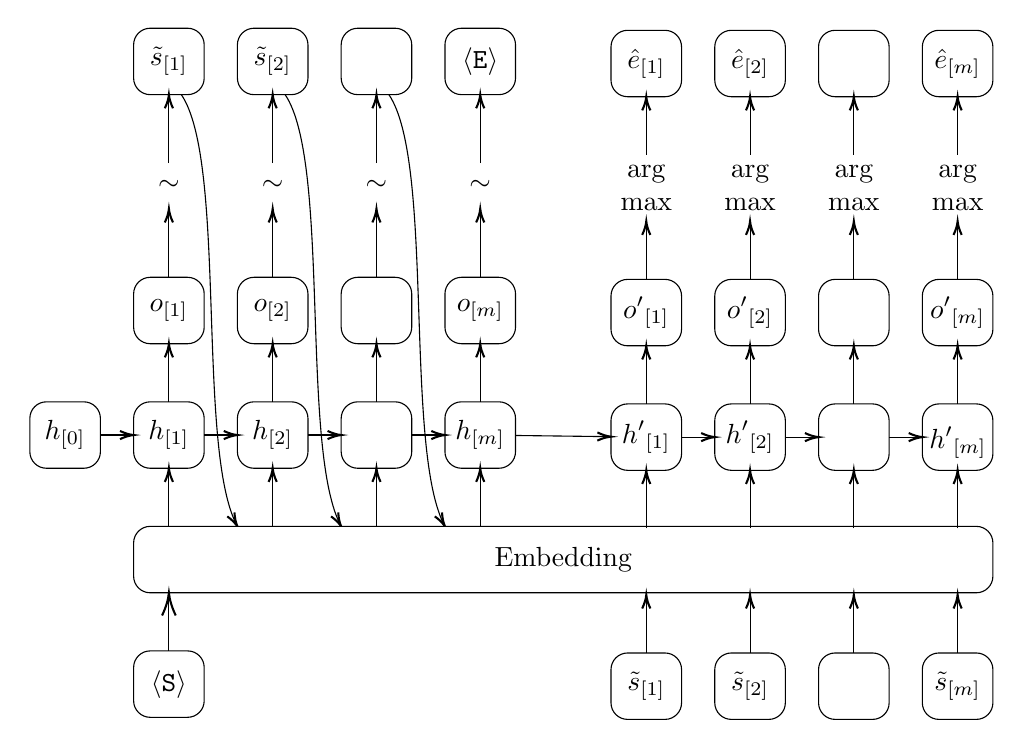
\begin{tikzpicture}[x=0.75pt,y=0.75pt,yscale=-1,xscale=1]
%uncomment if require: \path (0,355); %set diagram left start at 0, and has height of 355

%Curve Lines [id:da898021526375558]
\draw    (81,45) .. controls (102.77,77.16) and (88.54,212.5) .. (107.13,251.3) ;
\draw [shift={(108,253)}, rotate = 241.3] [color={rgb, 255:red, 0; green, 0; blue, 0 }  ][line width=0.75]    (6.56,-1.97) .. controls (4.17,-0.84) and (1.99,-0.18) .. (0,0) .. controls (1.99,0.18) and (4.17,0.84) .. (6.56,1.97)   ;
%Curve Lines [id:da8193603993553868]
\draw    (131,45) .. controls (152.77,77.16) and (138.54,212.5) .. (157.13,251.3) ;
\draw [shift={(158,253)}, rotate = 241.3] [color={rgb, 255:red, 0; green, 0; blue, 0 }  ][line width=0.75]    (6.56,-1.97) .. controls (4.17,-0.84) and (1.99,-0.18) .. (0,0) .. controls (1.99,0.18) and (4.17,0.84) .. (6.56,1.97)   ;
%Curve Lines [id:da9217609497584229]
\draw    (181,45) .. controls (202.77,77.16) and (188.54,212.5) .. (207.13,251.3) ;
\draw [shift={(208,253)}, rotate = 241.3] [color={rgb, 255:red, 0; green, 0; blue, 0 }  ][line width=0.75]    (6.56,-1.97) .. controls (4.17,-0.84) and (1.99,-0.18) .. (0,0) .. controls (1.99,0.18) and (4.17,0.84) .. (6.56,1.97)   ;

% Text Node
\draw  [fill={rgb, 255:red, 255; green, 255; blue, 255 }  ,fill opacity=1 ]  (58,261) .. controls (58,256.58) and (61.58,253) .. (66,253) -- (464,253) .. controls (468.42,253) and (472,256.58) .. (472,261) -- (472,277) .. controls (472,281.42) and (468.42,285) .. (464,285) -- (66,285) .. controls (61.58,285) and (58,281.42) .. (58,277) -- cycle  ;
\draw (265,269) node   [align=left] {\begin{minipage}[lt]{278.8pt}\setlength\topsep{0pt}
\begin{center}
Embedding
\end{center}

\end{minipage}};
% Text Node
\draw (75,269) node   [align=left] {\begin{minipage}[lt]{20.400000000000002pt}\setlength\topsep{0pt}
\begin{center}
\end{center}

\end{minipage}};
% Text Node
\draw (125,269) node   [align=left] {\begin{minipage}[lt]{20.400000000000002pt}\setlength\topsep{0pt}
\begin{center}
\end{center}

\end{minipage}};
% Text Node
\draw (175,269) node   [align=left] {\begin{minipage}[lt]{20.400000000000002pt}\setlength\topsep{0pt}
\begin{center}
\end{center}

\end{minipage}};
% Text Node
\draw (225,269) node   [align=left] {\begin{minipage}[lt]{20.400000000000002pt}\setlength\topsep{0pt}
\begin{center}
\end{center}

\end{minipage}};
% Text Node
\draw    (58,201) .. controls (58,196.58) and (61.58,193) .. (66,193) -- (84,193) .. controls (88.42,193) and (92,196.58) .. (92,201) -- (92,217) .. controls (92,221.42) and (88.42,225) .. (84,225) -- (66,225) .. controls (61.58,225) and (58,221.42) .. (58,217) -- cycle  ;
\draw (75,209) node   [align=left] {\begin{minipage}[lt]{20.400000000000002pt}\setlength\topsep{0pt}
\begin{center}
$\displaystyle \boldsymbol{h}_{[ 1]}$
\end{center}

\end{minipage}};
% Text Node
\draw    (108,201) .. controls (108,196.58) and (111.58,193) .. (116,193) -- (134,193) .. controls (138.42,193) and (142,196.58) .. (142,201) -- (142,217) .. controls (142,221.42) and (138.42,225) .. (134,225) -- (116,225) .. controls (111.58,225) and (108,221.42) .. (108,217) -- cycle  ;
\draw (125,209) node   [align=left] {\begin{minipage}[lt]{20.400000000000002pt}\setlength\topsep{0pt}
\begin{center}
$\displaystyle \boldsymbol{h}_{[ 2]}$
\end{center}

\end{minipage}};
% Text Node
\draw    (158,201) .. controls (158,196.58) and (161.58,193) .. (166,193) -- (184,193) .. controls (188.42,193) and (192,196.58) .. (192,201) -- (192,217) .. controls (192,221.42) and (188.42,225) .. (184,225) -- (166,225) .. controls (161.58,225) and (158,221.42) .. (158,217) -- cycle  ;
\draw (175,209) node   [align=left] {\begin{minipage}[lt]{20.400000000000002pt}\setlength\topsep{0pt}
\begin{center}
$\displaystyle \dotsc $
\end{center}

\end{minipage}};
% Text Node
\draw    (208,201) .. controls (208,196.58) and (211.58,193) .. (216,193) -- (234,193) .. controls (238.42,193) and (242,196.58) .. (242,201) -- (242,217) .. controls (242,221.42) and (238.42,225) .. (234,225) -- (216,225) .. controls (211.58,225) and (208,221.42) .. (208,217) -- cycle  ;
\draw (225,209) node   [align=left] {\begin{minipage}[lt]{20.400000000000002pt}\setlength\topsep{0pt}
\begin{center}
$\displaystyle \boldsymbol{h}_{[ m]}$
\end{center}

\end{minipage}};
% Text Node
\draw    (58,141) .. controls (58,136.58) and (61.58,133) .. (66,133) -- (84,133) .. controls (88.42,133) and (92,136.58) .. (92,141) -- (92,157) .. controls (92,161.42) and (88.42,165) .. (84,165) -- (66,165) .. controls (61.58,165) and (58,161.42) .. (58,157) -- cycle  ;
\draw (75,149) node   [align=left] {\begin{minipage}[lt]{20.400000000000002pt}\setlength\topsep{0pt}
\begin{center}
$\displaystyle \boldsymbol{o}_{[ 1]}$
\end{center}

\end{minipage}};
% Text Node
\draw    (108,141) .. controls (108,136.58) and (111.58,133) .. (116,133) -- (134,133) .. controls (138.42,133) and (142,136.58) .. (142,141) -- (142,157) .. controls (142,161.42) and (138.42,165) .. (134,165) -- (116,165) .. controls (111.58,165) and (108,161.42) .. (108,157) -- cycle  ;
\draw (125,149) node   [align=left] {\begin{minipage}[lt]{20.400000000000002pt}\setlength\topsep{0pt}
\begin{center}
$\displaystyle \boldsymbol{o}_{[ 2]}$
\end{center}

\end{minipage}};
% Text Node
\draw    (158,141) .. controls (158,136.58) and (161.58,133) .. (166,133) -- (184,133) .. controls (188.42,133) and (192,136.58) .. (192,141) -- (192,157) .. controls (192,161.42) and (188.42,165) .. (184,165) -- (166,165) .. controls (161.58,165) and (158,161.42) .. (158,157) -- cycle  ;
\draw (175,149) node   [align=left] {\begin{minipage}[lt]{20.400000000000002pt}\setlength\topsep{0pt}
\begin{center}
$\displaystyle \dotsc $
\end{center}

\end{minipage}};
% Text Node
\draw    (208,141) .. controls (208,136.58) and (211.58,133) .. (216,133) -- (234,133) .. controls (238.42,133) and (242,136.58) .. (242,141) -- (242,157) .. controls (242,161.42) and (238.42,165) .. (234,165) -- (216,165) .. controls (211.58,165) and (208,161.42) .. (208,157) -- cycle  ;
\draw (225,149) node   [align=left] {\begin{minipage}[lt]{20.400000000000002pt}\setlength\topsep{0pt}
\begin{center}
$\displaystyle \boldsymbol{o}_{[ m]}$
\end{center}

\end{minipage}};
% Text Node
\draw    (288,322) .. controls (288,317.58) and (291.58,314) .. (296,314) -- (314,314) .. controls (318.42,314) and (322,317.58) .. (322,322) -- (322,338) .. controls (322,342.42) and (318.42,346) .. (314,346) -- (296,346) .. controls (291.58,346) and (288,342.42) .. (288,338) -- cycle  ;
\draw (305,330) node   [align=left] {\begin{minipage}[lt]{20.400000000000002pt}\setlength\topsep{0pt}
\begin{center}
$\displaystyle \tilde{\boldsymbol{s}}_{[ 1]}$
\end{center}

\end{minipage}};
% Text Node
\draw (305,270) node   [align=left] {\begin{minipage}[lt]{20.400000000000002pt}\setlength\topsep{0pt}
\begin{center}
\end{center}

\end{minipage}};
% Text Node
\draw    (338,322) .. controls (338,317.58) and (341.58,314) .. (346,314) -- (364,314) .. controls (368.42,314) and (372,317.58) .. (372,322) -- (372,338) .. controls (372,342.42) and (368.42,346) .. (364,346) -- (346,346) .. controls (341.58,346) and (338,342.42) .. (338,338) -- cycle  ;
\draw (355,330) node   [align=left] {\begin{minipage}[lt]{20.400000000000002pt}\setlength\topsep{0pt}
\begin{center}
$\displaystyle \tilde{\boldsymbol{s}}_{[ 2]}$
\end{center}

\end{minipage}};
% Text Node
\draw    (388,322) .. controls (388,317.58) and (391.58,314) .. (396,314) -- (414,314) .. controls (418.42,314) and (422,317.58) .. (422,322) -- (422,338) .. controls (422,342.42) and (418.42,346) .. (414,346) -- (396,346) .. controls (391.58,346) and (388,342.42) .. (388,338) -- cycle  ;
\draw (405,330) node   [align=left] {\begin{minipage}[lt]{20.400000000000002pt}\setlength\topsep{0pt}
\begin{center}
$\displaystyle \dotsc $
\end{center}

\end{minipage}};
% Text Node
\draw    (438,322) .. controls (438,317.58) and (441.58,314) .. (446,314) -- (464,314) .. controls (468.42,314) and (472,317.58) .. (472,322) -- (472,338) .. controls (472,342.42) and (468.42,346) .. (464,346) -- (446,346) .. controls (441.58,346) and (438,342.42) .. (438,338) -- cycle  ;
\draw (455,330) node   [align=left] {\begin{minipage}[lt]{20.400000000000002pt}\setlength\topsep{0pt}
\begin{center}
$\displaystyle \tilde{\boldsymbol{s}}_{[ m]}$
\end{center}

\end{minipage}};
% Text Node
\draw (355,270) node   [align=left] {\begin{minipage}[lt]{20.400000000000002pt}\setlength\topsep{0pt}
\begin{center}
\end{center}

\end{minipage}};
% Text Node
\draw (405,270) node   [align=left] {\begin{minipage}[lt]{20.400000000000002pt}\setlength\topsep{0pt}
\begin{center}
\end{center}

\end{minipage}};
% Text Node
\draw (455,270) node   [align=left] {\begin{minipage}[lt]{20.400000000000002pt}\setlength\topsep{0pt}
\begin{center}
\end{center}

\end{minipage}};
% Text Node
\draw    (288,202) .. controls (288,197.58) and (291.58,194) .. (296,194) -- (314,194) .. controls (318.42,194) and (322,197.58) .. (322,202) -- (322,218) .. controls (322,222.42) and (318.42,226) .. (314,226) -- (296,226) .. controls (291.58,226) and (288,222.42) .. (288,218) -- cycle  ;
\draw (305,210) node   [align=left] {\begin{minipage}[lt]{20.400000000000002pt}\setlength\topsep{0pt}
\begin{center}
$\displaystyle \boldsymbol{h'}_{[ 1]}$
\end{center}

\end{minipage}};
% Text Node
\draw    (338,202) .. controls (338,197.58) and (341.58,194) .. (346,194) -- (364,194) .. controls (368.42,194) and (372,197.58) .. (372,202) -- (372,218) .. controls (372,222.42) and (368.42,226) .. (364,226) -- (346,226) .. controls (341.58,226) and (338,222.42) .. (338,218) -- cycle  ;
\draw (355,210) node   [align=left] {\begin{minipage}[lt]{20.400000000000002pt}\setlength\topsep{0pt}
\begin{center}
$\displaystyle \boldsymbol{h'}_{[ 2]}$
\end{center}

\end{minipage}};
% Text Node
\draw    (388,202) .. controls (388,197.58) and (391.58,194) .. (396,194) -- (414,194) .. controls (418.42,194) and (422,197.58) .. (422,202) -- (422,218) .. controls (422,222.42) and (418.42,226) .. (414,226) -- (396,226) .. controls (391.58,226) and (388,222.42) .. (388,218) -- cycle  ;
\draw (405,210) node   [align=left] {\begin{minipage}[lt]{20.400000000000002pt}\setlength\topsep{0pt}
\begin{center}
$\displaystyle \dotsc $
\end{center}

\end{minipage}};
% Text Node
\draw    (438,202) .. controls (438,197.58) and (441.58,194) .. (446,194) -- (464,194) .. controls (468.42,194) and (472,197.58) .. (472,202) -- (472,218) .. controls (472,222.42) and (468.42,226) .. (464,226) -- (446,226) .. controls (441.58,226) and (438,222.42) .. (438,218) -- cycle  ;
\draw (455,210) node   [align=left] {\begin{minipage}[lt]{20.400000000000002pt}\setlength\topsep{0pt}
\begin{center}
$\displaystyle \boldsymbol{h'}_{[ m]}$
\end{center}

\end{minipage}};
% Text Node
\draw    (288,142) .. controls (288,137.58) and (291.58,134) .. (296,134) -- (314,134) .. controls (318.42,134) and (322,137.58) .. (322,142) -- (322,158) .. controls (322,162.42) and (318.42,166) .. (314,166) -- (296,166) .. controls (291.58,166) and (288,162.42) .. (288,158) -- cycle  ;
\draw (305,150) node   [align=left] {\begin{minipage}[lt]{20.400000000000002pt}\setlength\topsep{0pt}
\begin{center}
$\displaystyle \boldsymbol{o'}_{[ 1]}$
\end{center}

\end{minipage}};
% Text Node
\draw    (338,142) .. controls (338,137.58) and (341.58,134) .. (346,134) -- (364,134) .. controls (368.42,134) and (372,137.58) .. (372,142) -- (372,158) .. controls (372,162.42) and (368.42,166) .. (364,166) -- (346,166) .. controls (341.58,166) and (338,162.42) .. (338,158) -- cycle  ;
\draw (355,150) node   [align=left] {\begin{minipage}[lt]{20.400000000000002pt}\setlength\topsep{0pt}
\begin{center}
$\displaystyle \boldsymbol{o'}_{[ 2]}$
\end{center}

\end{minipage}};
% Text Node
\draw    (388,142) .. controls (388,137.58) and (391.58,134) .. (396,134) -- (414,134) .. controls (418.42,134) and (422,137.58) .. (422,142) -- (422,158) .. controls (422,162.42) and (418.42,166) .. (414,166) -- (396,166) .. controls (391.58,166) and (388,162.42) .. (388,158) -- cycle  ;
\draw (405,150) node   [align=left] {\begin{minipage}[lt]{20.400000000000002pt}\setlength\topsep{0pt}
\begin{center}
$\displaystyle \dotsc $
\end{center}

\end{minipage}};
% Text Node
\draw    (438,142) .. controls (438,137.58) and (441.58,134) .. (446,134) -- (464,134) .. controls (468.42,134) and (472,137.58) .. (472,142) -- (472,158) .. controls (472,162.42) and (468.42,166) .. (464,166) -- (446,166) .. controls (441.58,166) and (438,162.42) .. (438,158) -- cycle  ;
\draw (455,150) node   [align=left] {\begin{minipage}[lt]{20.400000000000002pt}\setlength\topsep{0pt}
\begin{center}
$\displaystyle \boldsymbol{o'}_{[ m]}$
\end{center}

\end{minipage}};
% Text Node
\draw (75,89) node   [align=left] {\begin{minipage}[lt]{13.600000000000001pt}\setlength\topsep{0pt}
\begin{center}
$\displaystyle \sim $
\end{center}

\end{minipage}};
% Text Node
\draw (125,89) node   [align=left] {\begin{minipage}[lt]{13.600000000000001pt}\setlength\topsep{0pt}
\begin{center}
$\displaystyle \sim $
\end{center}

\end{minipage}};
% Text Node
\draw (175,89) node   [align=left] {\begin{minipage}[lt]{13.600000000000001pt}\setlength\topsep{0pt}
\begin{center}
$\displaystyle \sim $
\end{center}

\end{minipage}};
% Text Node
\draw (225,89) node   [align=left] {\begin{minipage}[lt]{13.600000000000001pt}\setlength\topsep{0pt}
\begin{center}
$\displaystyle \sim $
\end{center}

\end{minipage}};
% Text Node
\draw    (58,21) .. controls (58,16.58) and (61.58,13) .. (66,13) -- (84,13) .. controls (88.42,13) and (92,16.58) .. (92,21) -- (92,37) .. controls (92,41.42) and (88.42,45) .. (84,45) -- (66,45) .. controls (61.58,45) and (58,41.42) .. (58,37) -- cycle  ;
\draw (75,29) node   [align=left] {\begin{minipage}[lt]{20.400000000000002pt}\setlength\topsep{0pt}
\begin{center}
$\displaystyle \tilde{\boldsymbol{s}}_{[ 1]}$
\end{center}

\end{minipage}};
% Text Node
\draw    (108,21) .. controls (108,16.58) and (111.58,13) .. (116,13) -- (134,13) .. controls (138.42,13) and (142,16.58) .. (142,21) -- (142,37) .. controls (142,41.42) and (138.42,45) .. (134,45) -- (116,45) .. controls (111.58,45) and (108,41.42) .. (108,37) -- cycle  ;
\draw (125,29) node   [align=left] {\begin{minipage}[lt]{20.400000000000002pt}\setlength\topsep{0pt}
\begin{center}
$\displaystyle \tilde{\boldsymbol{s}}_{[ 2]}$
\end{center}

\end{minipage}};
% Text Node
\draw    (158,21) .. controls (158,16.58) and (161.58,13) .. (166,13) -- (184,13) .. controls (188.42,13) and (192,16.58) .. (192,21) -- (192,37) .. controls (192,41.42) and (188.42,45) .. (184,45) -- (166,45) .. controls (161.58,45) and (158,41.42) .. (158,37) -- cycle  ;
\draw (175,29) node   [align=left] {\begin{minipage}[lt]{20.400000000000002pt}\setlength\topsep{0pt}
\begin{center}
$\displaystyle \dotsc $
\end{center}

\end{minipage}};
% Text Node
\draw    (208,21) .. controls (208,16.58) and (211.58,13) .. (216,13) -- (234,13) .. controls (238.42,13) and (242,16.58) .. (242,21) -- (242,37) .. controls (242,41.42) and (238.42,45) .. (234,45) -- (216,45) .. controls (211.58,45) and (208,41.42) .. (208,37) -- cycle  ;
\draw (225,29) node   [align=left] {\begin{minipage}[lt]{20.400000000000002pt}\setlength\topsep{0pt}
\begin{center}
$\displaystyle \langle \mathtt{E} \rangle $
\end{center}

\end{minipage}};
% Text Node
\draw    (288,22) .. controls (288,17.58) and (291.58,14) .. (296,14) -- (314,14) .. controls (318.42,14) and (322,17.58) .. (322,22) -- (322,38) .. controls (322,42.42) and (318.42,46) .. (314,46) -- (296,46) .. controls (291.58,46) and (288,42.42) .. (288,38) -- cycle  ;
\draw (305,30) node   [align=left] {\begin{minipage}[lt]{20.400000000000002pt}\setlength\topsep{0pt}
\begin{center}
$\displaystyle \hat{\boldsymbol{e}}_{[ 1]}$
\end{center}

\end{minipage}};
% Text Node
\draw    (338,22) .. controls (338,17.58) and (341.58,14) .. (346,14) -- (364,14) .. controls (368.42,14) and (372,17.58) .. (372,22) -- (372,38) .. controls (372,42.42) and (368.42,46) .. (364,46) -- (346,46) .. controls (341.58,46) and (338,42.42) .. (338,38) -- cycle  ;
\draw (355,30) node   [align=left] {\begin{minipage}[lt]{20.400000000000002pt}\setlength\topsep{0pt}
\begin{center}
$\displaystyle \hat{\boldsymbol{e}}_{[ 2]}$
\end{center}

\end{minipage}};
% Text Node
\draw    (388,22) .. controls (388,17.58) and (391.58,14) .. (396,14) -- (414,14) .. controls (418.42,14) and (422,17.58) .. (422,22) -- (422,38) .. controls (422,42.42) and (418.42,46) .. (414,46) -- (396,46) .. controls (391.58,46) and (388,42.42) .. (388,38) -- cycle  ;
\draw (405,30) node   [align=left] {\begin{minipage}[lt]{20.400000000000002pt}\setlength\topsep{0pt}
\begin{center}
$\displaystyle \dotsc $
\end{center}

\end{minipage}};
% Text Node
\draw    (438,22) .. controls (438,17.58) and (441.58,14) .. (446,14) -- (464,14) .. controls (468.42,14) and (472,17.58) .. (472,22) -- (472,38) .. controls (472,42.42) and (468.42,46) .. (464,46) -- (446,46) .. controls (441.58,46) and (438,42.42) .. (438,38) -- cycle  ;
\draw (455,30) node   [align=left] {\begin{minipage}[lt]{20.400000000000002pt}\setlength\topsep{0pt}
\begin{center}
$\displaystyle \hat{\boldsymbol{e}}_{[ m]}$
\end{center}

\end{minipage}};
% Text Node
\draw    (8,201) .. controls (8,196.58) and (11.58,193) .. (16,193) -- (34,193) .. controls (38.42,193) and (42,196.58) .. (42,201) -- (42,217) .. controls (42,221.42) and (38.42,225) .. (34,225) -- (16,225) .. controls (11.58,225) and (8,221.42) .. (8,217) -- cycle  ;
\draw (25,209) node   [align=left] {\begin{minipage}[lt]{20.400000000000002pt}\setlength\topsep{0pt}
\begin{center}
$\displaystyle \boldsymbol{h}_{[ 0]}$
\end{center}

\end{minipage}};
% Text Node
\draw    (58,321) .. controls (58,316.58) and (61.58,313) .. (66,313) -- (84,313) .. controls (88.42,313) and (92,316.58) .. (92,321) -- (92,337) .. controls (92,341.42) and (88.42,345) .. (84,345) -- (66,345) .. controls (61.58,345) and (58,341.42) .. (58,337) -- cycle  ;
\draw (75,329) node   [align=left] {\begin{minipage}[lt]{20.400000000000002pt}\setlength\topsep{0pt}
\begin{center}
$\displaystyle \langle \mathtt{S} \rangle $
\end{center}

\end{minipage}};
% Text Node
\draw (305,90) node   [align=left] {\begin{minipage}[lt]{20.400000000000002pt}\setlength\topsep{0pt}
\begin{center}
arg\\max
\end{center}

\end{minipage}};
% Text Node
\draw (355,90) node   [align=left] {\begin{minipage}[lt]{20.400000000000002pt}\setlength\topsep{0pt}
\begin{center}
arg\\max
\end{center}

\end{minipage}};
% Text Node
\draw (405,90) node   [align=left] {\begin{minipage}[lt]{20.400000000000002pt}\setlength\topsep{0pt}
\begin{center}
arg\\max
\end{center}

\end{minipage}};
% Text Node
\draw (455,90) node   [align=left] {\begin{minipage}[lt]{20.400000000000002pt}\setlength\topsep{0pt}
\begin{center}
arg\\max
\end{center}

\end{minipage}};
% Connection
\draw    (305,314) -- (305,288) ;
\draw [shift={(305,286)}, rotate = 450] [color={rgb, 255:red, 0; green, 0; blue, 0 }  ][line width=0.75]    (6.56,-1.97) .. controls (4.17,-0.84) and (1.99,-0.18) .. (0,0) .. controls (1.99,0.18) and (4.17,0.84) .. (6.56,1.97)   ;
% Connection
\draw    (355,314) -- (355,288) ;
\draw [shift={(355,286)}, rotate = 450] [color={rgb, 255:red, 0; green, 0; blue, 0 }  ][line width=0.75]    (6.56,-1.97) .. controls (4.17,-0.84) and (1.99,-0.18) .. (0,0) .. controls (1.99,0.18) and (4.17,0.84) .. (6.56,1.97)   ;
% Connection
\draw    (405,314) -- (405,288) ;
\draw [shift={(405,286)}, rotate = 450] [color={rgb, 255:red, 0; green, 0; blue, 0 }  ][line width=0.75]    (6.56,-1.97) .. controls (4.17,-0.84) and (1.99,-0.18) .. (0,0) .. controls (1.99,0.18) and (4.17,0.84) .. (6.56,1.97)   ;
% Connection
\draw    (455,314) -- (455,288) ;
\draw [shift={(455,286)}, rotate = 450] [color={rgb, 255:red, 0; green, 0; blue, 0 }  ][line width=0.75]    (6.56,-1.97) .. controls (4.17,-0.84) and (1.99,-0.18) .. (0,0) .. controls (1.99,0.18) and (4.17,0.84) .. (6.56,1.97)   ;
% Connection
\draw    (75,253) -- (75,227) ;
\draw [shift={(75,225)}, rotate = 450] [color={rgb, 255:red, 0; green, 0; blue, 0 }  ][line width=0.75]    (6.56,-1.97) .. controls (4.17,-0.84) and (1.99,-0.18) .. (0,0) .. controls (1.99,0.18) and (4.17,0.84) .. (6.56,1.97)   ;
% Connection
\draw    (125,253) -- (125,227) ;
\draw [shift={(125,225)}, rotate = 450] [color={rgb, 255:red, 0; green, 0; blue, 0 }  ][line width=0.75]    (6.56,-1.97) .. controls (4.17,-0.84) and (1.99,-0.18) .. (0,0) .. controls (1.99,0.18) and (4.17,0.84) .. (6.56,1.97)   ;
% Connection
\draw    (175,253) -- (175,227) ;
\draw [shift={(175,225)}, rotate = 450] [color={rgb, 255:red, 0; green, 0; blue, 0 }  ][line width=0.75]    (6.56,-1.97) .. controls (4.17,-0.84) and (1.99,-0.18) .. (0,0) .. controls (1.99,0.18) and (4.17,0.84) .. (6.56,1.97)   ;
% Connection
\draw    (225,253) -- (225,227) ;
\draw [shift={(225,225)}, rotate = 450] [color={rgb, 255:red, 0; green, 0; blue, 0 }  ][line width=0.75]    (6.56,-1.97) .. controls (4.17,-0.84) and (1.99,-0.18) .. (0,0) .. controls (1.99,0.18) and (4.17,0.84) .. (6.56,1.97)   ;
% Connection
\draw    (305,254) -- (305,228) ;
\draw [shift={(305,226)}, rotate = 450] [color={rgb, 255:red, 0; green, 0; blue, 0 }  ][line width=0.75]    (6.56,-1.97) .. controls (4.17,-0.84) and (1.99,-0.18) .. (0,0) .. controls (1.99,0.18) and (4.17,0.84) .. (6.56,1.97)   ;
% Connection
\draw    (355,254) -- (355,228) ;
\draw [shift={(355,226)}, rotate = 450] [color={rgb, 255:red, 0; green, 0; blue, 0 }  ][line width=0.75]    (6.56,-1.97) .. controls (4.17,-0.84) and (1.99,-0.18) .. (0,0) .. controls (1.99,0.18) and (4.17,0.84) .. (6.56,1.97)   ;
% Connection
\draw    (405,254) -- (405,228) ;
\draw [shift={(405,226)}, rotate = 450] [color={rgb, 255:red, 0; green, 0; blue, 0 }  ][line width=0.75]    (6.56,-1.97) .. controls (4.17,-0.84) and (1.99,-0.18) .. (0,0) .. controls (1.99,0.18) and (4.17,0.84) .. (6.56,1.97)   ;
% Connection
\draw    (455,254) -- (455,228) ;
\draw [shift={(455,226)}, rotate = 450] [color={rgb, 255:red, 0; green, 0; blue, 0 }  ][line width=0.75]    (6.56,-1.97) .. controls (4.17,-0.84) and (1.99,-0.18) .. (0,0) .. controls (1.99,0.18) and (4.17,0.84) .. (6.56,1.97)   ;
% Connection
\draw    (92,209) -- (106,209) ;
\draw [shift={(108,209)}, rotate = 180] [color={rgb, 255:red, 0; green, 0; blue, 0 }  ][line width=0.75]    (6.56,-1.97) .. controls (4.17,-0.84) and (1.99,-0.18) .. (0,0) .. controls (1.99,0.18) and (4.17,0.84) .. (6.56,1.97)   ;
% Connection
\draw    (142,209) -- (156,209) ;
\draw [shift={(158,209)}, rotate = 180] [color={rgb, 255:red, 0; green, 0; blue, 0 }  ][line width=0.75]    (6.56,-1.97) .. controls (4.17,-0.84) and (1.99,-0.18) .. (0,0) .. controls (1.99,0.18) and (4.17,0.84) .. (6.56,1.97)   ;
% Connection
\draw    (192,209) -- (206,209) ;
\draw [shift={(208,209)}, rotate = 180] [color={rgb, 255:red, 0; green, 0; blue, 0 }  ][line width=0.75]    (6.56,-1.97) .. controls (4.17,-0.84) and (1.99,-0.18) .. (0,0) .. controls (1.99,0.18) and (4.17,0.84) .. (6.56,1.97)   ;
% Connection
\draw    (242,209.21) -- (286,209.76) ;
\draw [shift={(288,209.79)}, rotate = 180.72] [color={rgb, 255:red, 0; green, 0; blue, 0 }  ][line width=0.75]    (6.56,-1.97) .. controls (4.17,-0.84) and (1.99,-0.18) .. (0,0) .. controls (1.99,0.18) and (4.17,0.84) .. (6.56,1.97)   ;
% Connection
\draw    (322,210) -- (336,210) ;
\draw [shift={(338,210)}, rotate = 180] [color={rgb, 255:red, 0; green, 0; blue, 0 }  ][line width=0.75]    (6.56,-1.97) .. controls (4.17,-0.84) and (1.99,-0.18) .. (0,0) .. controls (1.99,0.18) and (4.17,0.84) .. (6.56,1.97)   ;
% Connection
\draw    (372,210) -- (386,210) ;
\draw [shift={(388,210)}, rotate = 180] [color={rgb, 255:red, 0; green, 0; blue, 0 }  ][line width=0.75]    (6.56,-1.97) .. controls (4.17,-0.84) and (1.99,-0.18) .. (0,0) .. controls (1.99,0.18) and (4.17,0.84) .. (6.56,1.97)   ;
% Connection
\draw    (422,210) -- (436,210) ;
\draw [shift={(438,210)}, rotate = 180] [color={rgb, 255:red, 0; green, 0; blue, 0 }  ][line width=0.75]    (6.56,-1.97) .. controls (4.17,-0.84) and (1.99,-0.18) .. (0,0) .. controls (1.99,0.18) and (4.17,0.84) .. (6.56,1.97)   ;
% Connection
\draw    (75,193) -- (75,167) ;
\draw [shift={(75,165)}, rotate = 450] [color={rgb, 255:red, 0; green, 0; blue, 0 }  ][line width=0.75]    (6.56,-1.97) .. controls (4.17,-0.84) and (1.99,-0.18) .. (0,0) .. controls (1.99,0.18) and (4.17,0.84) .. (6.56,1.97)   ;
% Connection
\draw    (125,193) -- (125,167) ;
\draw [shift={(125,165)}, rotate = 450] [color={rgb, 255:red, 0; green, 0; blue, 0 }  ][line width=0.75]    (6.56,-1.97) .. controls (4.17,-0.84) and (1.99,-0.18) .. (0,0) .. controls (1.99,0.18) and (4.17,0.84) .. (6.56,1.97)   ;
% Connection
\draw    (175,193) -- (175,167) ;
\draw [shift={(175,165)}, rotate = 450] [color={rgb, 255:red, 0; green, 0; blue, 0 }  ][line width=0.75]    (6.56,-1.97) .. controls (4.17,-0.84) and (1.99,-0.18) .. (0,0) .. controls (1.99,0.18) and (4.17,0.84) .. (6.56,1.97)   ;
% Connection
\draw    (225,193) -- (225,167) ;
\draw [shift={(225,165)}, rotate = 450] [color={rgb, 255:red, 0; green, 0; blue, 0 }  ][line width=0.75]    (6.56,-1.97) .. controls (4.17,-0.84) and (1.99,-0.18) .. (0,0) .. controls (1.99,0.18) and (4.17,0.84) .. (6.56,1.97)   ;
% Connection
\draw    (305,194) -- (305,168) ;
\draw [shift={(305,166)}, rotate = 450] [color={rgb, 255:red, 0; green, 0; blue, 0 }  ][line width=0.75]    (6.56,-1.97) .. controls (4.17,-0.84) and (1.99,-0.18) .. (0,0) .. controls (1.99,0.18) and (4.17,0.84) .. (6.56,1.97)   ;
% Connection
\draw    (355,194) -- (355,168) ;
\draw [shift={(355,166)}, rotate = 450] [color={rgb, 255:red, 0; green, 0; blue, 0 }  ][line width=0.75]    (6.56,-1.97) .. controls (4.17,-0.84) and (1.99,-0.18) .. (0,0) .. controls (1.99,0.18) and (4.17,0.84) .. (6.56,1.97)   ;
% Connection
\draw    (405,194) -- (405,168) ;
\draw [shift={(405,166)}, rotate = 450] [color={rgb, 255:red, 0; green, 0; blue, 0 }  ][line width=0.75]    (6.56,-1.97) .. controls (4.17,-0.84) and (1.99,-0.18) .. (0,0) .. controls (1.99,0.18) and (4.17,0.84) .. (6.56,1.97)   ;
% Connection
\draw    (455,194) -- (455,168) ;
\draw [shift={(455,166)}, rotate = 450] [color={rgb, 255:red, 0; green, 0; blue, 0 }  ][line width=0.75]    (6.56,-1.97) .. controls (4.17,-0.84) and (1.99,-0.18) .. (0,0) .. controls (1.99,0.18) and (4.17,0.84) .. (6.56,1.97)   ;
% Connection
\draw    (75,133) -- (75,102) ;
\draw [shift={(75,100)}, rotate = 450] [color={rgb, 255:red, 0; green, 0; blue, 0 }  ][line width=0.75]    (6.56,-1.97) .. controls (4.17,-0.84) and (1.99,-0.18) .. (0,0) .. controls (1.99,0.18) and (4.17,0.84) .. (6.56,1.97)   ;
% Connection
\draw    (125,133) -- (125,102) ;
\draw [shift={(125,100)}, rotate = 450] [color={rgb, 255:red, 0; green, 0; blue, 0 }  ][line width=0.75]    (6.56,-1.97) .. controls (4.17,-0.84) and (1.99,-0.18) .. (0,0) .. controls (1.99,0.18) and (4.17,0.84) .. (6.56,1.97)   ;
% Connection
\draw    (175,133) -- (175,102) ;
\draw [shift={(175,100)}, rotate = 450] [color={rgb, 255:red, 0; green, 0; blue, 0 }  ][line width=0.75]    (6.56,-1.97) .. controls (4.17,-0.84) and (1.99,-0.18) .. (0,0) .. controls (1.99,0.18) and (4.17,0.84) .. (6.56,1.97)   ;
% Connection
\draw    (225,133) -- (225,102) ;
\draw [shift={(225,100)}, rotate = 450] [color={rgb, 255:red, 0; green, 0; blue, 0 }  ][line width=0.75]    (6.56,-1.97) .. controls (4.17,-0.84) and (1.99,-0.18) .. (0,0) .. controls (1.99,0.18) and (4.17,0.84) .. (6.56,1.97)   ;
% Connection
\draw    (42,209) -- (56,209) ;
\draw [shift={(58,209)}, rotate = 180] [color={rgb, 255:red, 0; green, 0; blue, 0 }  ][line width=0.75]    (6.56,-1.97) .. controls (4.17,-0.84) and (1.99,-0.18) .. (0,0) .. controls (1.99,0.18) and (4.17,0.84) .. (6.56,1.97)   ;
% Connection
\draw    (75,313) -- (75,287) ;
\draw [shift={(75,285)}, rotate = 450] [color={rgb, 255:red, 0; green, 0; blue, 0 }  ][line width=0.75]    (10.93,-3.29) .. controls (6.95,-1.4) and (3.31,-0.3) .. (0,0) .. controls (3.31,0.3) and (6.95,1.4) .. (10.93,3.29)   ;
% Connection
\draw    (75,78) -- (75,47) ;
\draw [shift={(75,45)}, rotate = 450] [color={rgb, 255:red, 0; green, 0; blue, 0 }  ][line width=0.75]    (6.56,-1.97) .. controls (4.17,-0.84) and (1.99,-0.18) .. (0,0) .. controls (1.99,0.18) and (4.17,0.84) .. (6.56,1.97)   ;
% Connection
\draw    (125,78) -- (125,47) ;
\draw [shift={(125,45)}, rotate = 450] [color={rgb, 255:red, 0; green, 0; blue, 0 }  ][line width=0.75]    (6.56,-1.97) .. controls (4.17,-0.84) and (1.99,-0.18) .. (0,0) .. controls (1.99,0.18) and (4.17,0.84) .. (6.56,1.97)   ;
% Connection
\draw    (175,78) -- (175,47) ;
\draw [shift={(175,45)}, rotate = 450] [color={rgb, 255:red, 0; green, 0; blue, 0 }  ][line width=0.75]    (6.56,-1.97) .. controls (4.17,-0.84) and (1.99,-0.18) .. (0,0) .. controls (1.99,0.18) and (4.17,0.84) .. (6.56,1.97)   ;
% Connection
\draw    (225,78) -- (225,47) ;
\draw [shift={(225,45)}, rotate = 450] [color={rgb, 255:red, 0; green, 0; blue, 0 }  ][line width=0.75]    (6.56,-1.97) .. controls (4.17,-0.84) and (1.99,-0.18) .. (0,0) .. controls (1.99,0.18) and (4.17,0.84) .. (6.56,1.97)   ;
% Connection
\draw    (305,134) -- (305,108) ;
\draw [shift={(305,106)}, rotate = 450] [color={rgb, 255:red, 0; green, 0; blue, 0 }  ][line width=0.75]    (6.56,-1.97) .. controls (4.17,-0.84) and (1.99,-0.18) .. (0,0) .. controls (1.99,0.18) and (4.17,0.84) .. (6.56,1.97)   ;
% Connection
\draw    (355,134) -- (355,108) ;
\draw [shift={(355,106)}, rotate = 450] [color={rgb, 255:red, 0; green, 0; blue, 0 }  ][line width=0.75]    (6.56,-1.97) .. controls (4.17,-0.84) and (1.99,-0.18) .. (0,0) .. controls (1.99,0.18) and (4.17,0.84) .. (6.56,1.97)   ;
% Connection
\draw    (405,134) -- (405,108) ;
\draw [shift={(405,106)}, rotate = 450] [color={rgb, 255:red, 0; green, 0; blue, 0 }  ][line width=0.75]    (6.56,-1.97) .. controls (4.17,-0.84) and (1.99,-0.18) .. (0,0) .. controls (1.99,0.18) and (4.17,0.84) .. (6.56,1.97)   ;
% Connection
\draw    (455,134) -- (455,108) ;
\draw [shift={(455,106)}, rotate = 450] [color={rgb, 255:red, 0; green, 0; blue, 0 }  ][line width=0.75]    (6.56,-1.97) .. controls (4.17,-0.84) and (1.99,-0.18) .. (0,0) .. controls (1.99,0.18) and (4.17,0.84) .. (6.56,1.97)   ;
% Connection
\draw    (305,74) -- (305,48) ;
\draw [shift={(305,46)}, rotate = 450] [color={rgb, 255:red, 0; green, 0; blue, 0 }  ][line width=0.75]    (6.56,-1.97) .. controls (4.17,-0.84) and (1.99,-0.18) .. (0,0) .. controls (1.99,0.18) and (4.17,0.84) .. (6.56,1.97)   ;
% Connection
\draw    (355,74) -- (355,48) ;
\draw [shift={(355,46)}, rotate = 450] [color={rgb, 255:red, 0; green, 0; blue, 0 }  ][line width=0.75]    (6.56,-1.97) .. controls (4.17,-0.84) and (1.99,-0.18) .. (0,0) .. controls (1.99,0.18) and (4.17,0.84) .. (6.56,1.97)   ;
% Connection
\draw    (405,74) -- (405,48) ;
\draw [shift={(405,46)}, rotate = 450] [color={rgb, 255:red, 0; green, 0; blue, 0 }  ][line width=0.75]    (6.56,-1.97) .. controls (4.17,-0.84) and (1.99,-0.18) .. (0,0) .. controls (1.99,0.18) and (4.17,0.84) .. (6.56,1.97)   ;
% Connection
\draw    (455,74) -- (455,48) ;
\draw [shift={(455,46)}, rotate = 450] [color={rgb, 255:red, 0; green, 0; blue, 0 }  ][line width=0.75]    (6.56,-1.97) .. controls (4.17,-0.84) and (1.99,-0.18) .. (0,0) .. controls (1.99,0.18) and (4.17,0.84) .. (6.56,1.97)   ;

\end{tikzpicture}}
    \caption{Graph generation using the proposed model. The output of the network are two sequences: one is a stochastic sequence $\Vector{\tilde{s}}$ representing the starting sequence of the graph. The other is a deterministic ending sequence $\Vector{\hat{e}}$, predicted using $\Vector{\tilde{s}}$ as input. The two sequences are ultimately combined to produce the ordered edge sequence of a novel graph (not shown).}
    \label{fig:model-sampling}
\end{figure*}

\subsection{Implementation Details}\label{sec:implementation}
The model is implemented using the \texttt{PyTorch}\footnote{\url{https://github.com/marcopodda/grapher}} \cite{paszke2017pytorch} library; after an initial exploratory phase (not reported), some hyper-parameters (such as the number of recurrent layers) were fixed in advance. The other hyper-parameters are selected with an 80\%-20\% internal model selection. We choose among 32 and 64 for the embedding dimension $d$, 128 and 256 for the recurrent state size $h$. We apply a dropout layer to the embedding layer, whose rate is chosen between 0.25 and 0.35. As recurrent cells, we use 2 layers of Gated Recurrent Units (GRU) \cite{cho2014gru}. As regards the learning parameters, we use the Adam \cite{kingma2015adam} optimizer with learning rate of 0.001, halved every 200 epochs. We train all models for a maximum of 2000 epochs, applying early stopping whenever the loss starts to plateau (we found a suitable empirical threshold after running a number of exploratory training instances).

\section{Experiments}
Following, we detail the experiments to assess our model, describing the datasets used for learning, the baselines we compared to, and the framework used for evaluation.

\subsection{Datasets}\label{sec:datasets}
In our experiments, we evaluate our model on 3 synthetic datasets and 2 real-world datasets of molecular graphs. Every synthetic dataset represents graphs with particular node/edge dependencies. The rationale is to assess whether our approach is general enough to give good performances on very different graph distributions. Concretely, we use the following datasets:

\begin{itemize}
    \item LADDERS, a synthetic dataset of ladder graphs. We generate all possible ladder graphs having a number of nodes equal to $2n, n = 2, \ldots, 20$, and replicate them 10 times, resulting in a total size of 180 graphs. This dataset is inspired from the GRIDS dataset used in \citep{you2018graphrnn}. In our case, we use ladder graphs because they have a similar node degree distribution, while being computationally manageable. In this dataset, the model has to capture very strong dependencies: the nodes of a ladder graph have degree of 3, except nodes at the four corners, which have degree of two. Any graph that does not respect these dependencies is not a ladder graph. An example of ladder graph is shown in Figure \ref{fig:ladder};
    \item COMMUNITY, a synthetic dataset of graphs with two-community structure. Community graphs are composed of two densely connected clusters of nodes, which are weakly connected between themselves. Here, the model has to capture the community structure. Community dependencies are very common in biological settings: for example, densely connected communities in metabolic networks often represent functional groups (see \eg \citep{girvan2002commstructsocialbionet}). To create this dataset, we firstly generate two clique graphs of random size between $8 \leq N \leq 20$. We then remove some edges randomly from the two clusters with probability $0.4$, and then connect the two communities with 1 or 2 edges at random. The generated dataset is composed of 1000 graphs. This dataset is similar to the COMMUNITY dataset used in \citep{you2018graphrnn}, which unfortunately we could not reproduce. An example of community graph is shown in Figure \ref{fig:community};
    \item EGO, a dataset of ego networks extracted from the Citeseer dataset \citep{giles1998citeseer}. In this case, the model has to capture the presence of a focal node (the \quotes{ego} node), which is connected to the majority of nodes in the graph, while the other nodes (the \quotes{alter} nodes) have weaker connectivity. This dependency is typical of social networks, and can be modeled with the BA model for preferential attachment. To create the dataset, we extract all possible ego networks of radius 2 from the Citeseer dataset. Thus, the path length between the ego node and the alter nodes is at most 2. The total number of graphs in the dataset is 1719. An example of ego graph is shown in Figure \ref{fig:ego};
    \item TREES, a synthetic dataset of balanced and unbalanced ternary trees presented in \citep{bacciu2019baymixhidtreemarkovclus}. The dataset is composed of 780 ternary trees, of which one third is symmetric (\ie the number of nodes is almost identical in each subtree at the same level), one third left-asymmetric, and one third right-asymmetric. A left-asymmetric (right-asymmetric) tree is one where if the number of nodes in the leftmost (rightmost) position is greater than the number of nodes in the opposite position, whilst symmetric trees, have an almost equivalent number of nodes for each position. The dataset is divided into 600 trees for training (200 symmetric, 200 left-symmetric, 200 right-symmetric), and 180 trees for testing (60 symmetric, 60 left-symmetric, and 60 right-symmetric);
    \item ENZYMES, a subset of 436 graphs taken from the ENZYMES dataset \citep{schomburg2004enzymes} (see Section \ref{sec:comparison-datasets} for details);
    \item PROTEINS, a subset of 794 graphs taken from the Dobson and Doig dataset \citep{dobson2003dd} (see Section \ref{sec:comparison-datasets} for details). In these two last datasets, the model should capture patterns of connectivity typical of molecules, such as functional groups or aromatic rings.
\end{itemize}
All datasets have a number of nodes comprised between 4 and 40 (the only exception is TREES, where the number of nodes is comprised between 34 and 229), and a number of edges comprised between 2 and 130 (33 and 228, respectively, for TREES). Before training, we held out a portion of the dataset for testing purposes (except for TREES, where the split was provided in advance). In particular, for all datasets except LADDERS, we held out 30\% of graphs, and used them for evaluation. This held-out set acts as a random sample drawn from the corresponding unknown graph distribution.
\begin{figure*}[h!]
    \begin{subfigure}[b]{0.24\linewidth}
        \centering
        \resizebox{.35\textwidth}{!}{

\tikzset{every picture/.style={line width=0.75pt}} %set default line width to 0.75pt

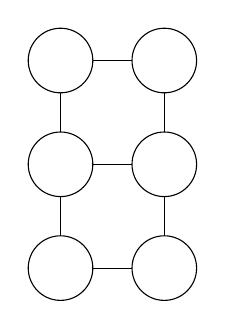
\begin{tikzpicture}[x=0.75pt,y=0.75pt,yscale=-1,xscale=1]
%uncomment if require: \path (0,166); %set diagram left start at 0, and has height of 166


% Text Node
\draw    (40, 30) circle [x radius= 15.56, y radius= 15.56]   ;
\draw (40,30) node   [align=left] {\begin{minipage}[lt]{13.600000000000001pt}\setlength\topsep{0pt}

\end{minipage}};
% Text Node
\draw    (90, 30) circle [x radius= 15.56, y radius= 15.56]   ;
\draw (90,30) node   [align=left] {\begin{minipage}[lt]{13.600000000000001pt}\setlength\topsep{0pt}

\end{minipage}};
% Text Node
\draw    (40, 80) circle [x radius= 15.56, y radius= 15.56]   ;
\draw (40,80) node   [align=left] {\begin{minipage}[lt]{13.600000000000001pt}\setlength\topsep{0pt}

\end{minipage}};
% Text Node
\draw    (90, 80) circle [x radius= 15.56, y radius= 15.56]   ;
\draw (90,80) node   [align=left] {\begin{minipage}[lt]{13.600000000000001pt}\setlength\topsep{0pt}

\end{minipage}};
% Text Node
\draw    (40, 130) circle [x radius= 15.56, y radius= 15.56]   ;
\draw (40,130) node   [align=left] {\begin{minipage}[lt]{13.600000000000001pt}\setlength\topsep{0pt}

\end{minipage}};
% Text Node
\draw    (90, 130) circle [x radius= 15.56, y radius= 15.56]   ;
\draw (90,130) node   [align=left] {\begin{minipage}[lt]{13.600000000000001pt}\setlength\topsep{0pt}

\end{minipage}};
% Connection
\draw    (55.56,30) -- (74.44,30) ;
% Connection
\draw    (40,45.56) -- (40,64.44) ;
% Connection
\draw    (90,45.56) -- (90,64.44) ;
% Connection
\draw    (40,95.56) -- (40,114.44) ;
% Connection
\draw    (90,95.56) -- (90,114.44) ;
% Connection
\draw    (55.56,130) -- (74.44,130) ;
% Connection
\draw    (55.56,80) -- (74.44,80) ;

\end{tikzpicture}}
        \caption{LADDERS.}
        \label{fig:ladder}
    \end{subfigure}
    \begin{subfigure}[b]{0.24\linewidth}
        \centering
        \resizebox{.8\textwidth}{!}{

\tikzset{every picture/.style={line width=0.75pt}} %set default line width to 0.75pt

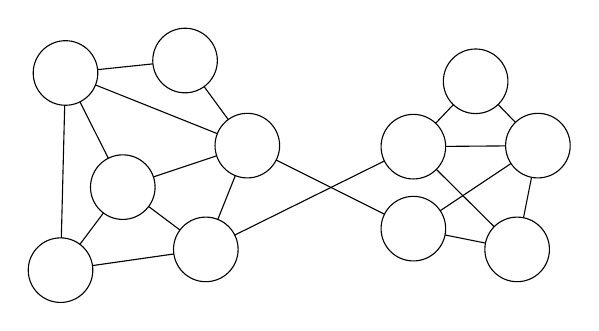
\begin{tikzpicture}[x=0.75pt,y=0.75pt,yscale=-1,xscale=1]
%uncomment if require: \path (0,158); %set diagram left start at 0, and has height of 158


% Text Node
\draw    (32.4, 26) circle [x radius= 15.56, y radius= 15.56]   ;
\draw (32.4,26) node   [align=left] {\begin{minipage}[lt]{13.600000000000001pt}\setlength\topsep{0pt}

\end{minipage}};
% Text Node
\draw    (90, 20) circle [x radius= 15.56, y radius= 15.56]   ;
\draw (90,20) node   [align=left] {\begin{minipage}[lt]{13.600000000000001pt}\setlength\topsep{0pt}

\end{minipage}};
% Text Node
\draw    (60, 81) circle [x radius= 15.56, y radius= 15.56]   ;
\draw (60,81) node   [align=left] {\begin{minipage}[lt]{13.600000000000001pt}\setlength\topsep{0pt}

\end{minipage}};
% Text Node
\draw    (120, 61) circle [x radius= 15.56, y radius= 15.56]   ;
\draw (120,61) node   [align=left] {\begin{minipage}[lt]{13.600000000000001pt}\setlength\topsep{0pt}

\end{minipage}};
% Text Node
\draw    (30, 121) circle [x radius= 15.56, y radius= 15.56]   ;
\draw (30,121) node   [align=left] {\begin{minipage}[lt]{13.600000000000001pt}\setlength\topsep{0pt}

\end{minipage}};
% Text Node
\draw    (100, 111) circle [x radius= 15.56, y radius= 15.56]   ;
\draw (100,111) node   [align=left] {\begin{minipage}[lt]{13.600000000000001pt}\setlength\topsep{0pt}

\end{minipage}};
% Text Node
\draw    (230, 30) circle [x radius= 15.56, y radius= 15.56]   ;
\draw (230,30) node   [align=left] {\begin{minipage}[lt]{13.600000000000001pt}\setlength\topsep{0pt}

\end{minipage}};
% Text Node
\draw    (200, 61.5) circle [x radius= 15.56, y radius= 15.56]   ;
\draw (200,61.5) node   [align=left] {\begin{minipage}[lt]{13.600000000000001pt}\setlength\topsep{0pt}

\end{minipage}};
% Text Node
\draw    (260, 61) circle [x radius= 15.56, y radius= 15.56]   ;
\draw (260,61) node   [align=left] {\begin{minipage}[lt]{13.600000000000001pt}\setlength\topsep{0pt}

\end{minipage}};
% Text Node
\draw    (200, 101) circle [x radius= 15.56, y radius= 15.56]   ;
\draw (200,101) node   [align=left] {\begin{minipage}[lt]{13.600000000000001pt}\setlength\topsep{0pt}

\end{minipage}};
% Text Node
\draw    (250, 111) circle [x radius= 15.56, y radius= 15.56]   ;
\draw (250,111) node   [align=left] {\begin{minipage}[lt]{13.600000000000001pt}\setlength\topsep{0pt}

\end{minipage}};
% Connection
\draw    (219.27,41.26) -- (210.73,50.24) ;
% Connection
\draw    (240.82,41.18) -- (249.18,49.82) ;
% Connection
\draw    (211.06,72.44) -- (238.94,100.06) ;
% Connection
\draw    (247.05,69.63) -- (212.95,92.37) ;
% Connection
\draw    (215.26,104.05) -- (234.74,107.95) ;
% Connection
\draw    (253.05,95.74) -- (256.95,76.26) ;
% Connection
\draw    (186.06,68.4) -- (113.94,104.1) ;
% Connection
\draw    (114.22,75.45) -- (105.78,96.55) ;
% Connection
\draw    (110.81,48.44) -- (99.19,32.56) ;
% Connection
\draw    (105.55,55.23) -- (46.85,31.77) ;
% Connection
\draw    (32.01,41.55) -- (30.39,105.45) ;
% Connection
\draw    (39.38,39.91) -- (53.02,67.09) ;
% Connection
\draw    (47.87,24.39) -- (74.53,21.61) ;
% Connection
\draw    (50.67,93.45) -- (39.33,108.55) ;
% Connection
\draw    (45.4,118.8) -- (84.6,113.2) ;
% Connection
\draw    (72.45,90.33) -- (87.55,101.67) ;
% Connection
\draw    (74.76,76.08) -- (105.24,65.92) ;
% Connection
\draw    (186.08,94.04) -- (133.92,67.96) ;
% Connection
\draw    (215.56,61.37) -- (244.44,61.13) ;

\end{tikzpicture}}
        \caption{COMMUNITY.}
        \label{fig:community}
    \end{subfigure}
    \begin{subfigure}[b]{0.24\linewidth}
        \centering
        \resizebox{.5\textwidth}{!}{

\tikzset{every picture/.style={line width=0.75pt}} %set default line width to 0.75pt

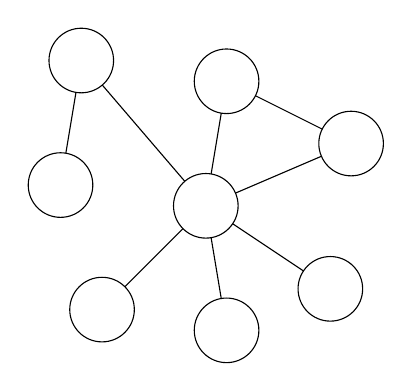
\begin{tikzpicture}[x=0.75pt,y=0.75pt,yscale=-1,xscale=1]
%uncomment if require: \path (0,194); %set diagram left start at 0, and has height of 194


% Text Node
\draw    (40, 30) circle [x radius= 15.56, y radius= 15.56]   ;
\draw (40,30) node   [align=left] {\begin{minipage}[lt]{13.600000000000001pt}\setlength\topsep{0pt}

\end{minipage}};
% Text Node
\draw    (100, 100) circle [x radius= 15.56, y radius= 15.56]   ;
\draw (100,100) node   [align=left] {\begin{minipage}[lt]{13.600000000000001pt}\setlength\topsep{0pt}

\end{minipage}};
% Text Node
\draw    (110, 40) circle [x radius= 15.56, y radius= 15.56]   ;
\draw (110,40) node   [align=left] {\begin{minipage}[lt]{13.600000000000001pt}\setlength\topsep{0pt}

\end{minipage}};
% Text Node
\draw    (170, 70) circle [x radius= 15.56, y radius= 15.56]   ;
\draw (170,70) node   [align=left] {\begin{minipage}[lt]{13.600000000000001pt}\setlength\topsep{0pt}

\end{minipage}};
% Text Node
\draw    (160, 140) circle [x radius= 15.56, y radius= 15.56]   ;
\draw (160,140) node   [align=left] {\begin{minipage}[lt]{13.600000000000001pt}\setlength\topsep{0pt}

\end{minipage}};
% Text Node
\draw    (110, 160) circle [x radius= 15.56, y radius= 15.56]   ;
\draw (110,160) node   [align=left] {\begin{minipage}[lt]{13.600000000000001pt}\setlength\topsep{0pt}

\end{minipage}};
% Text Node
\draw    (50, 150) circle [x radius= 15.56, y radius= 15.56]   ;
\draw (50,150) node   [align=left] {\begin{minipage}[lt]{13.600000000000001pt}\setlength\topsep{0pt}

\end{minipage}};
% Text Node
\draw    (30, 90) circle [x radius= 15.56, y radius= 15.56]   ;
\draw (30,90) node   [align=left] {\begin{minipage}[lt]{13.600000000000001pt}\setlength\topsep{0pt}

\end{minipage}};
% Connection
\draw    (89.88,88.19) -- (50.12,41.81) ;
% Connection
\draw    (89,111) -- (61,139) ;
% Connection
\draw    (102.56,115.35) -- (107.44,144.65) ;
% Connection
\draw    (112.95,108.63) -- (147.05,131.37) ;
% Connection
\draw    (114.3,93.87) -- (155.7,76.13) ;
% Connection
\draw    (102.56,84.65) -- (107.44,55.35) ;
% Connection
\draw    (123.92,46.96) -- (156.08,63.04) ;
% Connection
\draw    (37.44,45.35) -- (32.56,74.65) ;

\end{tikzpicture}}
        \caption{EGO.}
        \label{fig:ego}
    \end{subfigure}
    \begin{subfigure}[b]{0.24\linewidth}
        \centering
        \resizebox{.8\textwidth}{!}{

\tikzset{every picture/.style={line width=0.75pt}} %set default line width to 0.75pt

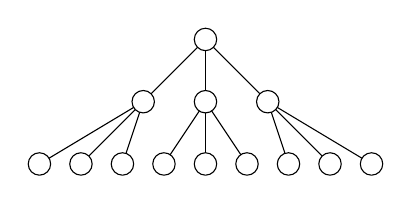
\begin{tikzpicture}[x=0.75pt,y=0.75pt,yscale=-1,xscale=1]
%uncomment if require: \path (0,300); %set diagram left start at 0, and has height of 300

%Straight Lines [id:da9885008986945643]
\draw    (114.6,34.6) -- (84.6,64.6) ;
%Straight Lines [id:da38066189494457126]
\draw    (84.6,64.6) -- (54.6,94.6) ;
%Straight Lines [id:da2388873036095942]
\draw    (84.6,64.6) -- (34.6,94.6) ;
%Straight Lines [id:da7229881469916373]
\draw    (84.6,64.6) -- (74.6,94.6) ;
%Straight Lines [id:da8983437299511077]
\draw    (114.6,34.6) -- (114.6,64.6) ;
%Straight Lines [id:da20426881992453816]
\draw    (114.6,34.6) -- (144.6,64.6) ;
%Straight Lines [id:da9928781316973885]
\draw    (114.6,64.6) -- (94.6,94.6) ;
%Straight Lines [id:da8503157507351102]
\draw    (144.6,64.6) -- (154.6,94.6) ;
%Straight Lines [id:da8375785947637939]
\draw    (144.6,64.6) -- (174.6,94.6) ;
%Straight Lines [id:da27683220373171546]
\draw    (144.6,64.6) -- (194.6,94.6) ;
%Straight Lines [id:da3424697297455832]
\draw    (114.6,64.6) -- (114.6,94.6) ;
%Straight Lines [id:da4700990532526734]
\draw    (114.6,64.6) -- (134.6,94.6) ;
%Shape: Circle [id:dp32353221475411176]
\draw  [fill={rgb, 255:red, 255; green, 255; blue, 255 }  ,fill opacity=1 ] (79.2,64.6) .. controls (79.2,61.62) and (81.62,59.2) .. (84.6,59.2) .. controls (87.58,59.2) and (90,61.62) .. (90,64.6) .. controls (90,67.58) and (87.58,70) .. (84.6,70) .. controls (81.62,70) and (79.2,67.58) .. (79.2,64.6) -- cycle ;
%Shape: Circle [id:dp6199501442233117]
\draw  [fill={rgb, 255:red, 255; green, 255; blue, 255 }  ,fill opacity=1 ] (109.2,64.6) .. controls (109.2,61.62) and (111.62,59.2) .. (114.6,59.2) .. controls (117.58,59.2) and (120,61.62) .. (120,64.6) .. controls (120,67.58) and (117.58,70) .. (114.6,70) .. controls (111.62,70) and (109.2,67.58) .. (109.2,64.6) -- cycle ;
%Shape: Circle [id:dp684335680256791]
\draw  [fill={rgb, 255:red, 255; green, 255; blue, 255 }  ,fill opacity=1 ] (139.2,64.6) .. controls (139.2,61.62) and (141.62,59.2) .. (144.6,59.2) .. controls (147.58,59.2) and (150,61.62) .. (150,64.6) .. controls (150,67.58) and (147.58,70) .. (144.6,70) .. controls (141.62,70) and (139.2,67.58) .. (139.2,64.6) -- cycle ;
%Shape: Circle [id:dp476261986912492]
\draw  [fill={rgb, 255:red, 255; green, 255; blue, 255 }  ,fill opacity=1 ] (109.2,34.6) .. controls (109.2,31.62) and (111.62,29.2) .. (114.6,29.2) .. controls (117.58,29.2) and (120,31.62) .. (120,34.6) .. controls (120,37.58) and (117.58,40) .. (114.6,40) .. controls (111.62,40) and (109.2,37.58) .. (109.2,34.6) -- cycle ;
%Shape: Circle [id:dp3402330352740246]
\draw  [fill={rgb, 255:red, 255; green, 255; blue, 255 }  ,fill opacity=1 ] (29.2,94.6) .. controls (29.2,91.62) and (31.62,89.2) .. (34.6,89.2) .. controls (37.58,89.2) and (40,91.62) .. (40,94.6) .. controls (40,97.58) and (37.58,100) .. (34.6,100) .. controls (31.62,100) and (29.2,97.58) .. (29.2,94.6) -- cycle ;
%Shape: Circle [id:dp5238406995823643]
\draw  [fill={rgb, 255:red, 255; green, 255; blue, 255 }  ,fill opacity=1 ] (49.2,94.6) .. controls (49.2,91.62) and (51.62,89.2) .. (54.6,89.2) .. controls (57.58,89.2) and (60,91.62) .. (60,94.6) .. controls (60,97.58) and (57.58,100) .. (54.6,100) .. controls (51.62,100) and (49.2,97.58) .. (49.2,94.6) -- cycle ;
%Shape: Circle [id:dp37074906375151917]
\draw  [fill={rgb, 255:red, 255; green, 255; blue, 255 }  ,fill opacity=1 ] (69.2,94.6) .. controls (69.2,91.62) and (71.62,89.2) .. (74.6,89.2) .. controls (77.58,89.2) and (80,91.62) .. (80,94.6) .. controls (80,97.58) and (77.58,100) .. (74.6,100) .. controls (71.62,100) and (69.2,97.58) .. (69.2,94.6) -- cycle ;
%Shape: Circle [id:dp35726516168084443]
\draw  [fill={rgb, 255:red, 255; green, 255; blue, 255 }  ,fill opacity=1 ] (89.2,94.6) .. controls (89.2,91.62) and (91.62,89.2) .. (94.6,89.2) .. controls (97.58,89.2) and (100,91.62) .. (100,94.6) .. controls (100,97.58) and (97.58,100) .. (94.6,100) .. controls (91.62,100) and (89.2,97.58) .. (89.2,94.6) -- cycle ;
%Shape: Circle [id:dp5697367388204451]
\draw  [fill={rgb, 255:red, 255; green, 255; blue, 255 }  ,fill opacity=1 ] (109.2,94.6) .. controls (109.2,91.62) and (111.62,89.2) .. (114.6,89.2) .. controls (117.58,89.2) and (120,91.62) .. (120,94.6) .. controls (120,97.58) and (117.58,100) .. (114.6,100) .. controls (111.62,100) and (109.2,97.58) .. (109.2,94.6) -- cycle ;
%Shape: Circle [id:dp833509817631223]
\draw  [fill={rgb, 255:red, 255; green, 255; blue, 255 }  ,fill opacity=1 ] (129.2,94.6) .. controls (129.2,91.62) and (131.62,89.2) .. (134.6,89.2) .. controls (137.58,89.2) and (140,91.62) .. (140,94.6) .. controls (140,97.58) and (137.58,100) .. (134.6,100) .. controls (131.62,100) and (129.2,97.58) .. (129.2,94.6) -- cycle ;
%Shape: Circle [id:dp6035032605527935]
\draw  [fill={rgb, 255:red, 255; green, 255; blue, 255 }  ,fill opacity=1 ] (149.2,94.6) .. controls (149.2,91.62) and (151.62,89.2) .. (154.6,89.2) .. controls (157.58,89.2) and (160,91.62) .. (160,94.6) .. controls (160,97.58) and (157.58,100) .. (154.6,100) .. controls (151.62,100) and (149.2,97.58) .. (149.2,94.6) -- cycle ;
%Shape: Circle [id:dp4284418130247485]
\draw  [fill={rgb, 255:red, 255; green, 255; blue, 255 }  ,fill opacity=1 ] (169.2,94.6) .. controls (169.2,91.62) and (171.62,89.2) .. (174.6,89.2) .. controls (177.58,89.2) and (180,91.62) .. (180,94.6) .. controls (180,97.58) and (177.58,100) .. (174.6,100) .. controls (171.62,100) and (169.2,97.58) .. (169.2,94.6) -- cycle ;
%Shape: Circle [id:dp12689826995017484]
\draw  [fill={rgb, 255:red, 255; green, 255; blue, 255 }  ,fill opacity=1 ] (189.2,94.6) .. controls (189.2,91.62) and (191.62,89.2) .. (194.6,89.2) .. controls (197.58,89.2) and (200,91.62) .. (200,94.6) .. controls (200,97.58) and (197.58,100) .. (194.6,100) .. controls (191.62,100) and (189.2,97.58) .. (189.2,94.6) -- cycle ;




\end{tikzpicture}}
        \caption{TREES.}
        \label{fig:btree}
    \end{subfigure}
    \caption{Examples of the synthetic graphs used for the evaluation.}
    \label{fig:synthetic-graphs}
\end{figure*}
We also considered experimenting with two other graph families, namely cycles and complete graphs. However, we ultimately decided not to for two main reasons. Firstly, the number of unlabeled cycles and complete graphs is fixed, (exactly 1 for a given number of nodes). In the case of complete graphs especially, the connectivity of each graph is quadratic in the number of nodes, which would have made a dataset of reasonable size computationally unmanageable. Secondly, cyclic and pseudo-complete sub-structures are already represented in the pool of datasets chosen: for example, ladder graphs are made of overlapping cycles, while the community graphs in the COMMUNITY dataset are densely connected (and thus very similar to complete graphs). For these reasons, we decided to carry on the experiments only with the above-mentioned datasets.

For the LADDERS dataset, we held out 10\% of graphs in a stratified fashion. In practice, the held-out set for LADDERS is composed of the same 18 unique ladder graphs found in the training set. To motivate this choice, let us clarify the role of the LADDERS dataset: its purpose is not to evaluate generalization capability, but to show that adaptive models can overfit hard node/edge dependencies among nodes, while non-adaptive models (such as the ER and BA models) cannot. The statistics of the datasets used for evaluation are presented in Table \ref{tab:generation-datasets}.

\begin{table}[h!]
    \footnotesize
    \centering
    \caption{Statistics of datasets used in the experiments.}
    \label{tab:generation-datasets}
    \begin{tabular}{lcccc}
        \toprule
         \textbf{Dataset} & \textbf{No. of graphs} & \textbf{Test size} & \textbf{Avg. no. of nodes} & \textbf{Avg. no. of edges}\\
         \midrule
         LADDERS & 180 & 18 & 21.00 & 29.50 \\
         COMMUNITY & 1000 & 300 & 24.38 & 88.58 \\
         EGO & 1719 & 516 & 13.02 & 18.51 \\
         ENZYMES & 436 & 130 & 26.14 & 51.16 \\
         PROTEINS & 794 & 238 & 20.49 & 38.67 \\
        \bottomrule
    \end{tabular}
\end{table}

\subsection{Baselines}
We compare against four baseline models. Two of them are classical generative models of graphs coming from graph theory literature, namely the ER and BA models. The rationale behind this choice is to assess whether our model is able to perform better than random models that model graph connectivity independently (ER), or consider just one simple edge dependency (BA, where the probability of an edge is a function of the node degree).

The ER model has two parameters: $n$, the number of nodes of the graph to be generated, and $P$, the probability of adding an edge between a pair of nodes. The generative process of the ER model can be described informally as follows: first, pick $n$, then, for each possible pair of nodes, sample a Bernoulli random variable with probability $P$, and connect the two nodes according to the sampled value. We sample $n$ from the empirical distribution of the number of nodes in the datasets, and choose $P$ from a grid of values. The best value of $P$ is obtained by minimizing the earth mover distance between the empirical distribution and the generated distribution of graph properties.

Similarly, the BA model has two parameters: $n$, the number of nodes of the graph to be generated, and $M$, a maximum number of nodes a node can be connected to. The generative process for a BA graph proceeds incrementally: given an already formed graph, add a new node and connect it (or not) to at most $M$ nodes with probability proportional to the nodes' degree. In our experiments, the two parameters of the BA model are optimized similarly to the ER model.

Besides graph theory baselines, we also compare to a strong Deep-Learning based generative baseline. In particular, we choose the GraphRNN model of \citet{you2018graphrnn}, which holds state-of-the-art performances in the graph generation task. We implemented the model according to the original code repository provided by the authors, following their implementation and their hyper-parameters configuration closely.

Lastly, we introduce a third baseline model, a recurrent neural network with GRU cells that is trained to predict the adjacency matrix of the graph one entry at a time. We call this baseline GRU-B(aseline) from now on. It is arguably the simplest model one can come up with to model graph generation in a recurrent fashion, with the limitation that it has to sample $n(n-1)/2$ entries to fully specify the adjacency matrix of an undirected graph with $n$ nodes, making it susceptible to learning issues induced by long-term dependencies \citep{bengio1994learninglongtermdependenciesdifficult}. Clearly, even though Deep-Learning based, this baseline has purposely limited expressiveness with respect of our model and GraphRNN.

\subsection{Evaluation Framework}
We assess our model against the baselines following the quantitative and qualitative evaluation principles described in Section \ref{sec:evaluation-generative-graphs}. The experiments are described as follows:
\begin{itemize}
    \item the first experiment consists in evaluating the model quantitatively. To confidently detect overfitting, we choose to generate samples larger than the training set. Specifically, we generate two samples of size 1000 and 5000 from all the candidates. For each generated sample, we measure their novelty (with respect to the training set) and their uniqueness (with respect to the same generated graphs). Despite using chemical datasets (ENZYMES and PROTEINS), we do not evaluate chemical validity because we are concerned about generating unlabeled graphs; thus, chemical validity cannot be assessed in our case. Finally, we also measure the time that each model takes to generate the 5000 graph sample;
    \item the second experiment is of qualitative nature. In practice, we assess how much the generated samples resemble a random sample from the graph distribution of reference. The assessment consists of extracting local and global statistics from the generated graphs, and comparing their distribution to that of the test graphs. The local statistics evaluated are Degree Distribution (DD), Clustering Coefficient (CC), and Orbit Counts (OC). For the global statistics, we choose Betweenness Centrality (BC) and Neighborhood Subgraph Pairwise Distance Kernel (NSPDK) \cite{costa2010nspdk}. Given a graph statistics, the discrepancy between the generated and reference distributions is computed as follows. Initially, a vector of statistics is extracted for each graph, and its length is equalized to 100 by fitting a histogram to its values. Then, the histograms are summed across all the samples of the generated graphs and the reference graphs, respectively. Finally, the \gls{kld} between the two resulting vectors is computed. The only exception is NSPDK, where we compute the Maximum Mean Discrepancy \cite{gretton2012mmdkernel} instead. Since the NSPDK only works with labelled graphs, we use node degrees as labels. All the calculations are repeated 10 times, each time using a different generated sample. In the following tables, the mean and the standard deviation of these 10 runs is reported.
\end{itemize}

\section{Results}
Here, we present the results of our experiments. We divide the analysis of the results into a quantitative and qualitative sections for readability purposes.

\subsection{Quantitative Analysis}
Table \ref{tab:graph-quantitative} shows the results of our quantitative experiments. The ER model achieves the best performances in the LADDERS and COMMUNITY datasets: this was expected, since the model produces random graphs that are very likely to be different from the training sample. Similarly, the BA model generates graphs whose structure is radically different from graphs coming from these two datasets by construction. In the EGO dataset, both models score poorly with respect to the competitors. We argue that this result is due to the nature of the EGO dataset, which is composed of graphs with very weak connectivity (except for the ego nodes) and a very low number of cycles. With such characteristics, it is easier for a random model to produce duplicates or overfit the training sample, just by setting the parameters that regulate connectivity to small values.
\begin{table}[h!]
    \footnotesize
    \centering
    \caption{Results of the quantitative analysis of the generated samples. In the leftmost column, both the metric of interest as well as the sample size (either 1000 or 5000) is specified. Best performances are bolded.}
    \label{tab:graph-quantitative}
    \renewcommand{\arraystretch}{1.2}
    \begin{tabular}{lcccccccc}
        \toprule
         \textbf{Dataset} & \textbf{Metric} & \textbf{ER} & \textbf{BA} & \textbf{GRU-B} & \textbf{GraphRNN} & \textbf{Ours} \\
         \midrule
          & Novelty@1000              & 0.98  & \textbf{1.00} & 0.66  & 0.97   & 0.99\\
          & Novelty@5000              & 0.99  & \textbf{1.00} & 0.71  & 0.96   & 0.99\\
          LADDERS & Uniqueness@1000   & \textbf{0.98}  & 0.86 & 0.17  & 0.26   & 0.22\\
          & Uniqueness@5000           & \textbf{0.86}  & 0.72 & 0.06  & 0.08   & 0.07\\
          & Time@5000                 & $<$1s & 1s   & 6m32s & 17m06s & 3m38s\\
         \midrule
          & Novelty@1000              & \textbf{1.00} & \textbf{1.00} & \textbf{1.00}  & \textbf{1.00}   & \textbf{1.00}\\
          & Novelty@5000              & \textbf{1.00} & \textbf{1.00} & \textbf{1.00}  & \textbf{1.00}   & \textbf{1.00}\\
          COMMUNITY & Uniqueness@1000 & \textbf{1.00} & \textbf{1.00} & \textbf{1.00}  & \textbf{1.00}   & \textbf{1.00}\\
          & Uniqueness@5000           & \textbf{1.00} & \textbf{1.00} & 0.99  & \textbf{1.00}   & \textbf{1.00}\\
          & Time@5000                 & 3s   & 5s   & 7m25s & 52m26s & 8m58s\\
         \midrule
          & Novelty@1000              & 0.69 & 0.74 & 0.62  & 0.74     & \textbf{0.96}\\
          & Novelty@5000              & 0.73 & 0.82 & 0.58  & 0.76     & \textbf{0.92}\\
          EGO & Uniqueness@1000       & 0.76 & 0.72 & 0.85  & 0.94     & \textbf{0.97}\\
          & Uniqueness@5000           & 0.65 & 0.61 & 0.64  & 0.87     & \textbf{0.91}\\
          & Time@5000                 & 1s   & 1s   & 6m01s & 1h10m16s & 3m23s\\
        \midrule
          & Novelty@1000              & \textbf{1.00} & \textbf{1.00} & \textbf{1.00}   & 0.99     & \textbf{1.00}\\
          & Novelty@5000              & \textbf{1.00} & \textbf{1.00} & \textbf{1.00}   & 0.99     & \textbf{1.00}\\
          TREES & Uniqueness@1000     & \textbf{1.00} & \textbf{1.00} & 0.89   & 0.94     & 0.88\\
          & Uniqueness@5000           & 0.98 & \textbf{1.00} & 0.64   & 0.89     & 0.70\\
          & Time@5000                 & 8s   & 8s   & 22m43s & 2h38m53s & 16m39s\\
         \midrule
          & Novelty@1000              & \textbf{1.00} & \textbf{1.00} & 0.99 & 0.95    & \textbf{1.00}\\
          & Novelty@5000              & \textbf{1.00} & \textbf{1.00} & 0.99 & 0.95    & \textbf{1.00}\\
          ENZYMES & Uniqueness@1000   & \textbf{1.00} & \textbf{1.00} & 0.98 & \textbf{1.00}    & \textbf{1.00}\\
          & Uniqueness@5000           & \textbf{1.00} & \textbf{1.00} & 0.81  & 0.97   & 0.92\\
          & Time@5000                 & 3s   & 3s   & 7m19s & 52m24s & 4m41s\\
        \midrule
          & Novelty@1000              & 0.98  & \textbf{1.00} & 0.90  & 0.75   & 0.95\\
          & Novelty@5000              & 0.98  & \textbf{1.00} & 0.91  & 0.76   & 0.96\\
          PROTEINS & Uniqueness@1000   & \textbf{0.98}  & 0.93 & 0.95  & 0.93   & 0.83\\
          & Uniqueness@5000           & \textbf{0.97}  & 0.92 & 0.77  & 0.84   & 0.65\\
          & Time@5000                 & $<$1s & 4s   & 6m29s & 54m07s & 3m44s\\
          \bottomrule
    \end{tabular}
\end{table}
In contrast, our model and GraphRNN consistently generate graphs with high novelty and uniqueness rates in almost all scenarios. The only exception to this trend is the LADDERS dataset, where both our model and GraphRNN overfit (they tend to generate the same graphs over and over), while the ER and BA models perform excellently. Again, these high scores imply that the ER and BA are unable to replicate the structures of these datasets.

The GRU-B model greatly under-performs in several datasets. From this result alone, one could legitimately infer that the model is not generalizing to unseen adjacency matrices. However, the qualitative analysis and the high value of the training loss (not shown) suggest that the model cannot perform any better. This provides evidence that a simple recurrent model such as GRU-B, at least in this form, is not well suited for the task of graph generation.

Our model and GraphRNN obtain excellent novelty and uniqueness scores in every dataset except LADDERS. Again, the poor scores in the LADDERS dataset indicate that they are able to overfit ladder graphs. Our model is the most consistent across all datasets, obtaining a score of at least 0.88 (except for the LADDERS dataset). When the sample size is large, both models tend to produce higher rates of duplicate graphs, which was again expected since the largest sample size exceeds the size of the training set.

Note how all models obtain a perfect score in the COMMUNITY dataset. This can be explained by considering the nature of the COMMUNITY dataset, whose graphs are essentially composed by two random graphs weakly connected among each other. Thus, since generating a graph from that distribution is very similar to generating two strongly connected components weakly connected together, samples are highly likely to be different from each other.

As regards sampling time, random models are the fastest during generation; this was expected, since they have only 2 parameters, while all RNN-based models have a larger number of parameters. Among the RNN-based models, our model is the fastest at generating new samples. One exception is the COMMUNITY dataset, where however it elapses only 1.5 minutes more than the winning model, GRU-B. In contrast, the GraphRNN model has sampling times 5 to 20 times slower than our model. For completeness, however, we report that while we sampled from the GraphRNN model with batch size of 1 to achieve a fair comparison, its implementation allows to drawing samples in batches, greatly speeding up the process.

% Table \ref{tab:graph-quantitative-rank} shows the mean rank of the models for each considered metric (except time), averaged over all datasets. More precisely, for a given metric, we collect the scores of all models on that particular metric and sort the corresponding vector in descending order from highest to lowest score. The order of the vector is the corresponding rank. The ranks are finally averaged across all datasets, to provide a measure of how models behave globally. The results show that the BA model has the highest mean rank as regards novelty on a sample size of 1000, while GraphRNN has the highest mean rank as regards novelty on a sample of 5000. Our model obtains the highest mean rank on uniqueness, on both sample sizes.
% \begin{table}[h!]
    \footnotesize
    \centering
    \caption{Mean ranks on all considered quantitative metrics except time, obtained by the examined models over all datasets. Best performances of models based on RNNs are bolded.}
    \label{tab:graph-quantitative-rank}
    \renewcommand{\arraystretch}{1.2}
    \begin{tabular}{cccccccc}
          \toprule
          \textbf{Metric} & \textbf{ER} & \textbf{BA} & \textbf{GRU-B} & \textbf{GraphRNN} & \textbf{Ours} \\
          \midrule
          Novelty@1000    & $3.00$ & $2.60$ & $3.20$ & $3.20$          & $\textbf{3.00}$\\
          Novelty@5000    & $3.00$ & $2.60$          & $4.00$ & $\textbf{2.40}$ & $3.00$\\
          Uniqueness@1000 & $2.60$ & $3.40$          & $3.20$ & $3.40$          & $\textbf{2.40}$\\
          Uniqueness@5000 & $2.60$ & $4.00$          & $3.40$ & $2.80$          & $\textbf{2.20}$\\
          \bottomrule
    \end{tabular}
\end{table}

\subsection{Qualitative Analysis}\label{sec:qualitative-analysis}
Table \ref{tab:graph-qualitative} shows the results of the qualitative evaluation of the models. Since we are measuring discrepancies between distributions of graph statistics, we remark that lower values indicate better fit. It can be clearly seen how random models are unable to learn complex dependencies, scoring poorly on all datasets in every considered metric. One exception is the TREES dataset, where the ER model obtains the best KLD for the CC metric.
\begin{table}[h!]
    \scriptsize
    \caption{Results of the qualitative analysis of the generated samples. The three metrics considered are KLDs calculated on Average Degree Distribution (ADD), Average Clustering Coefficient (ACC), and Average Orbit Count (AOD). Best performances are bolded.}
    \label{tab:graph-qualitative}
    \renewcommand{\arraystretch}{1.2}
    \makebox[\textwidth]{
    \begin{tabular}{lcccccc}
        \toprule
        \textbf{Dataset} & \textbf{Metric} & \textbf{ER} & \textbf{BA} & \textbf{GRU-B} & \textbf{GraphRNN} & \textbf{Ours} \\
        \midrule
          & DD           & 1.873 (0.134) & 0.945 (0.047) & 1.098 (0.162) & 0.035 (0.003) & \textbf{0.013} (0.003)\\
          & CC           & \textbf{0.000} (0.000) & 0.195 (0.029) & 0.004 (0.005) & \textbf{0.000} (0.000) & \textbf{0.000} (0.000)\\
LADDERS   & OC           & 1.853 (0.026) & 0.136 (0.022) & 0.026 (0.006) & \textbf{0.000} (0.000) & \textbf{0.000} (0.000)\\
          & BC           & 6.281 (0.877) & 1.756 (0.584) & 6.461 (1.447) & \textbf{0.566} (0.062) & 0.762 (0.180)\\
          & NSPDK        & 0.744 (0.007) & 0.569 (0.020) & 0.604 (0.110) & 0.139 (0.007) & \textbf{0.056} (0.022)\\
        \midrule
          & DD           & 0.353 (0.002) & 1.149 (0.080) & 0.167 (0.004) & 0.075 (0.000) & \textbf{0.013} (0.000)\\
          & CC           & 0.312 (0.031) & 1.643 (0.189) & 0.181 (0.012) & \textbf{0.074} (0.001) & 0.101 (0.011)\\
COMMUNITY & OC           & 0.073 (0.000) & 0.055 (0.001) & 0.006 (0.000) & \textbf{0.001} (0.000) & 0.013 (0.002)\\
          & BC           & 1.543 (0.039) & 2.642 (0.021) & 0.228 (0.032) & 0.311 (0.063) & \textbf{0.038} (0.005)\\
          & NSPDK        & 0.072 (0.001) & 0.156 (0.003) & 0.056 (0.001) & \textbf{0.009} (0.000) & \textbf{0.009} (0.000)\\
        \midrule
          & DD           & 0.723 (0.005) & 0.587 (0.004) & 0.244 (0.000) & 0.046 (0.001) & \textbf{0.029} (0.000)\\
          & CC           & 0.414 (0.002) & 0.698 (0.069) & 0.411 (0.005) & 0.194 (0.001) & \textbf{0.090} (0.011)\\
EGO       & OC           & 0.121 (0.001) & 0.384 (0.000) & 0.124 (0.001) & 0.009 (0.001) & \textbf{0.002} (0.000)\\
          & BC           & 1.100 (0.021) & 0.735 (0.020) & 0.127 (0.010) & 0.282 (0.024) & \textbf{0.096} (0.001)\\
          & NSPDK        & 0.098 (0.001) & 0.038 (0.000) & 0.009 (0.000) & \textbf{0.014} (0.001) & \textbf{0.016} (0.001)\\
        \midrule
          & DD           & 0.729 (0.011) & 0.810 (0.004) & 0.797 (0.005) & \textbf{0.036} (0.002) & 0.078 (0.002)\\
          & CC           & \textbf{0.000} (0.000) & 0.026 (0.001) & 0.128 (0.003) & \textbf{0.000} (0.000) & \textbf{0.000} (0.000)\\
TREES     & OC           & 0.418 (0.023) & 0.017 (0.000) & 0.081 (0.004) & \textbf{0.000} (0.000) & 0.001 (0.000)\\
          & BC           & 0.201 (0.003) & 0.754 (0.055) & 0.137 (0.003) & 0.170 (0.009) & \textbf{0.056} (0.008)\\
          & NSPDK        & 0.597 (0.004) & 0.718 (0.003) & 0.605 (0.011) & \textbf{0.022} (0.001) & 0.042 (0.004)\\
        \midrule
          & DD           & 1.124 (0.046) & 1.761 (0.045) & 0.475 (0.005) & 0.026 (0.003) & 0.040 (0.002)\\
          & CC           & 0.781 (0.003) & 1.680 (0.076) & 0.531 (0.051) & \textbf{0.113} (0.019) & \textbf{0.128} (0.037)\\
ENZYMES   & OC           & 0.218 (0.005) & 0.197 (0.001) & 0.022 (0.004) & \textbf{0.008} (0.001) & \textbf{0.005} (0.002)\\
          & BC           & 2.784 (0.066) & 5.753 (0.470) & 0.201 (0.031) & 0.086 (0.008) & \textbf{0.062} (0.006)\\
          & NSPDK        & 0.177 (0.006) & 0.235 (0.005) & 0.104 (0.003) & \textbf{0.015} (0.001) & 0.021 (0.001)\\
        \midrule
          & DD           & 1.224 (0.041) & 1.643 (0.033) & 0.532 (0.014) & \textbf{0.012} (0.003) & \textbf{0.018} (0.003)\\
          & CC           & 0.829 (0.010) & 1.264 (0.030) & 0.413 (0.026) & \textbf{0.043} (0.006) & 0.056 (0.005)\\
PROTEINS  & OC           & 0.256 (0.005) & 0.226 (0.004) & 0.020 (0.002) & \textbf{0.007} (0.004) & \textbf{0.002} (0.000)\\
          & BC           & 2.084 (0.255) & 3.735 (0.156) & 0.167 (0.040) & \textbf{0.023} (0.008) & 0.048 (0.005)\\
          & NSPDK        & 0.176 (0.004) & 0.172 (0.007) & 0.102 (0.002) & \textbf{0.008} (0.000) & \textbf{0.017} (0.000)\\
        \bottomrule

    \end{tabular}}
\end{table}
The GRU-B model struggles in almost every metric across all datasets. This reinforces the argument made with the quantitative analysis, \ie that this model suffers from limited expressiveness. Among all models, GraphRNN and ours perform consistently at the state of the art as regards the quality of generated graphs. In most cases, they perform indistinguishably. Notably, our model outperforms GraphRNN on every metric in the EGO dataset. Notice the low scores achieved by the two models on the global graph statistics (BC and NSPDK), which indicate that they are both able to learn the global structure of the graph, independently from the dataset they are trained on. To summarize the performances of the models, in Table \ref{tab:graph-qualitative-rank} we report the mean rank of all models. To rank the models, we first order the metrics by increasing score, collect the position of each model in the rank, and average across the datasets. Our model and GraphRNN perform almost indistinguishably when compared across all datasets.
\begin{table}[h!]
    \footnotesize
    \centering
    \caption{Mean ranks obtained on the evaluated qualitative metrics by the examined models over all datasets. Best performances are bolded.}
    \label{tab:graph-qualitative-rank}
    \renewcommand{\arraystretch}{1.2}
    \begin{tabular}{cccccccc}
          \toprule
          \textbf{Metric} & \textbf{ER} & \textbf{BA} & \textbf{GRU-B} & \textbf{GRNN} & \textbf{Ours} \\
          \midrule
          ADD    & $4.40$ & $4.60$ & $2.60$ & $2.00$ & $\textbf{1.40}$\\
          ACC    & $4.40$ & $4.00$ & $2.80$ & $2.40$ & $\textbf{1.40}$\\
          AOC    & $4.00$ & $3.80$ & $3.00$ & $2.20$ & $\textbf{2.00}$\\
          \bottomrule
    \end{tabular}
\end{table}
In Figure \ref{fig:distributions} we show graphically how well the generated samples match the empirical distribution of graph statistics across the datasets. We only consider four metrics (DD, CC, OC, and BC), for which histograms are available, fitting them with a Kernel Density Estimator (KDE) for visual comparison. The plots show that our model and GraphRNN well approximate the test sample statistics.
\begin{figure}[h!]
\centering
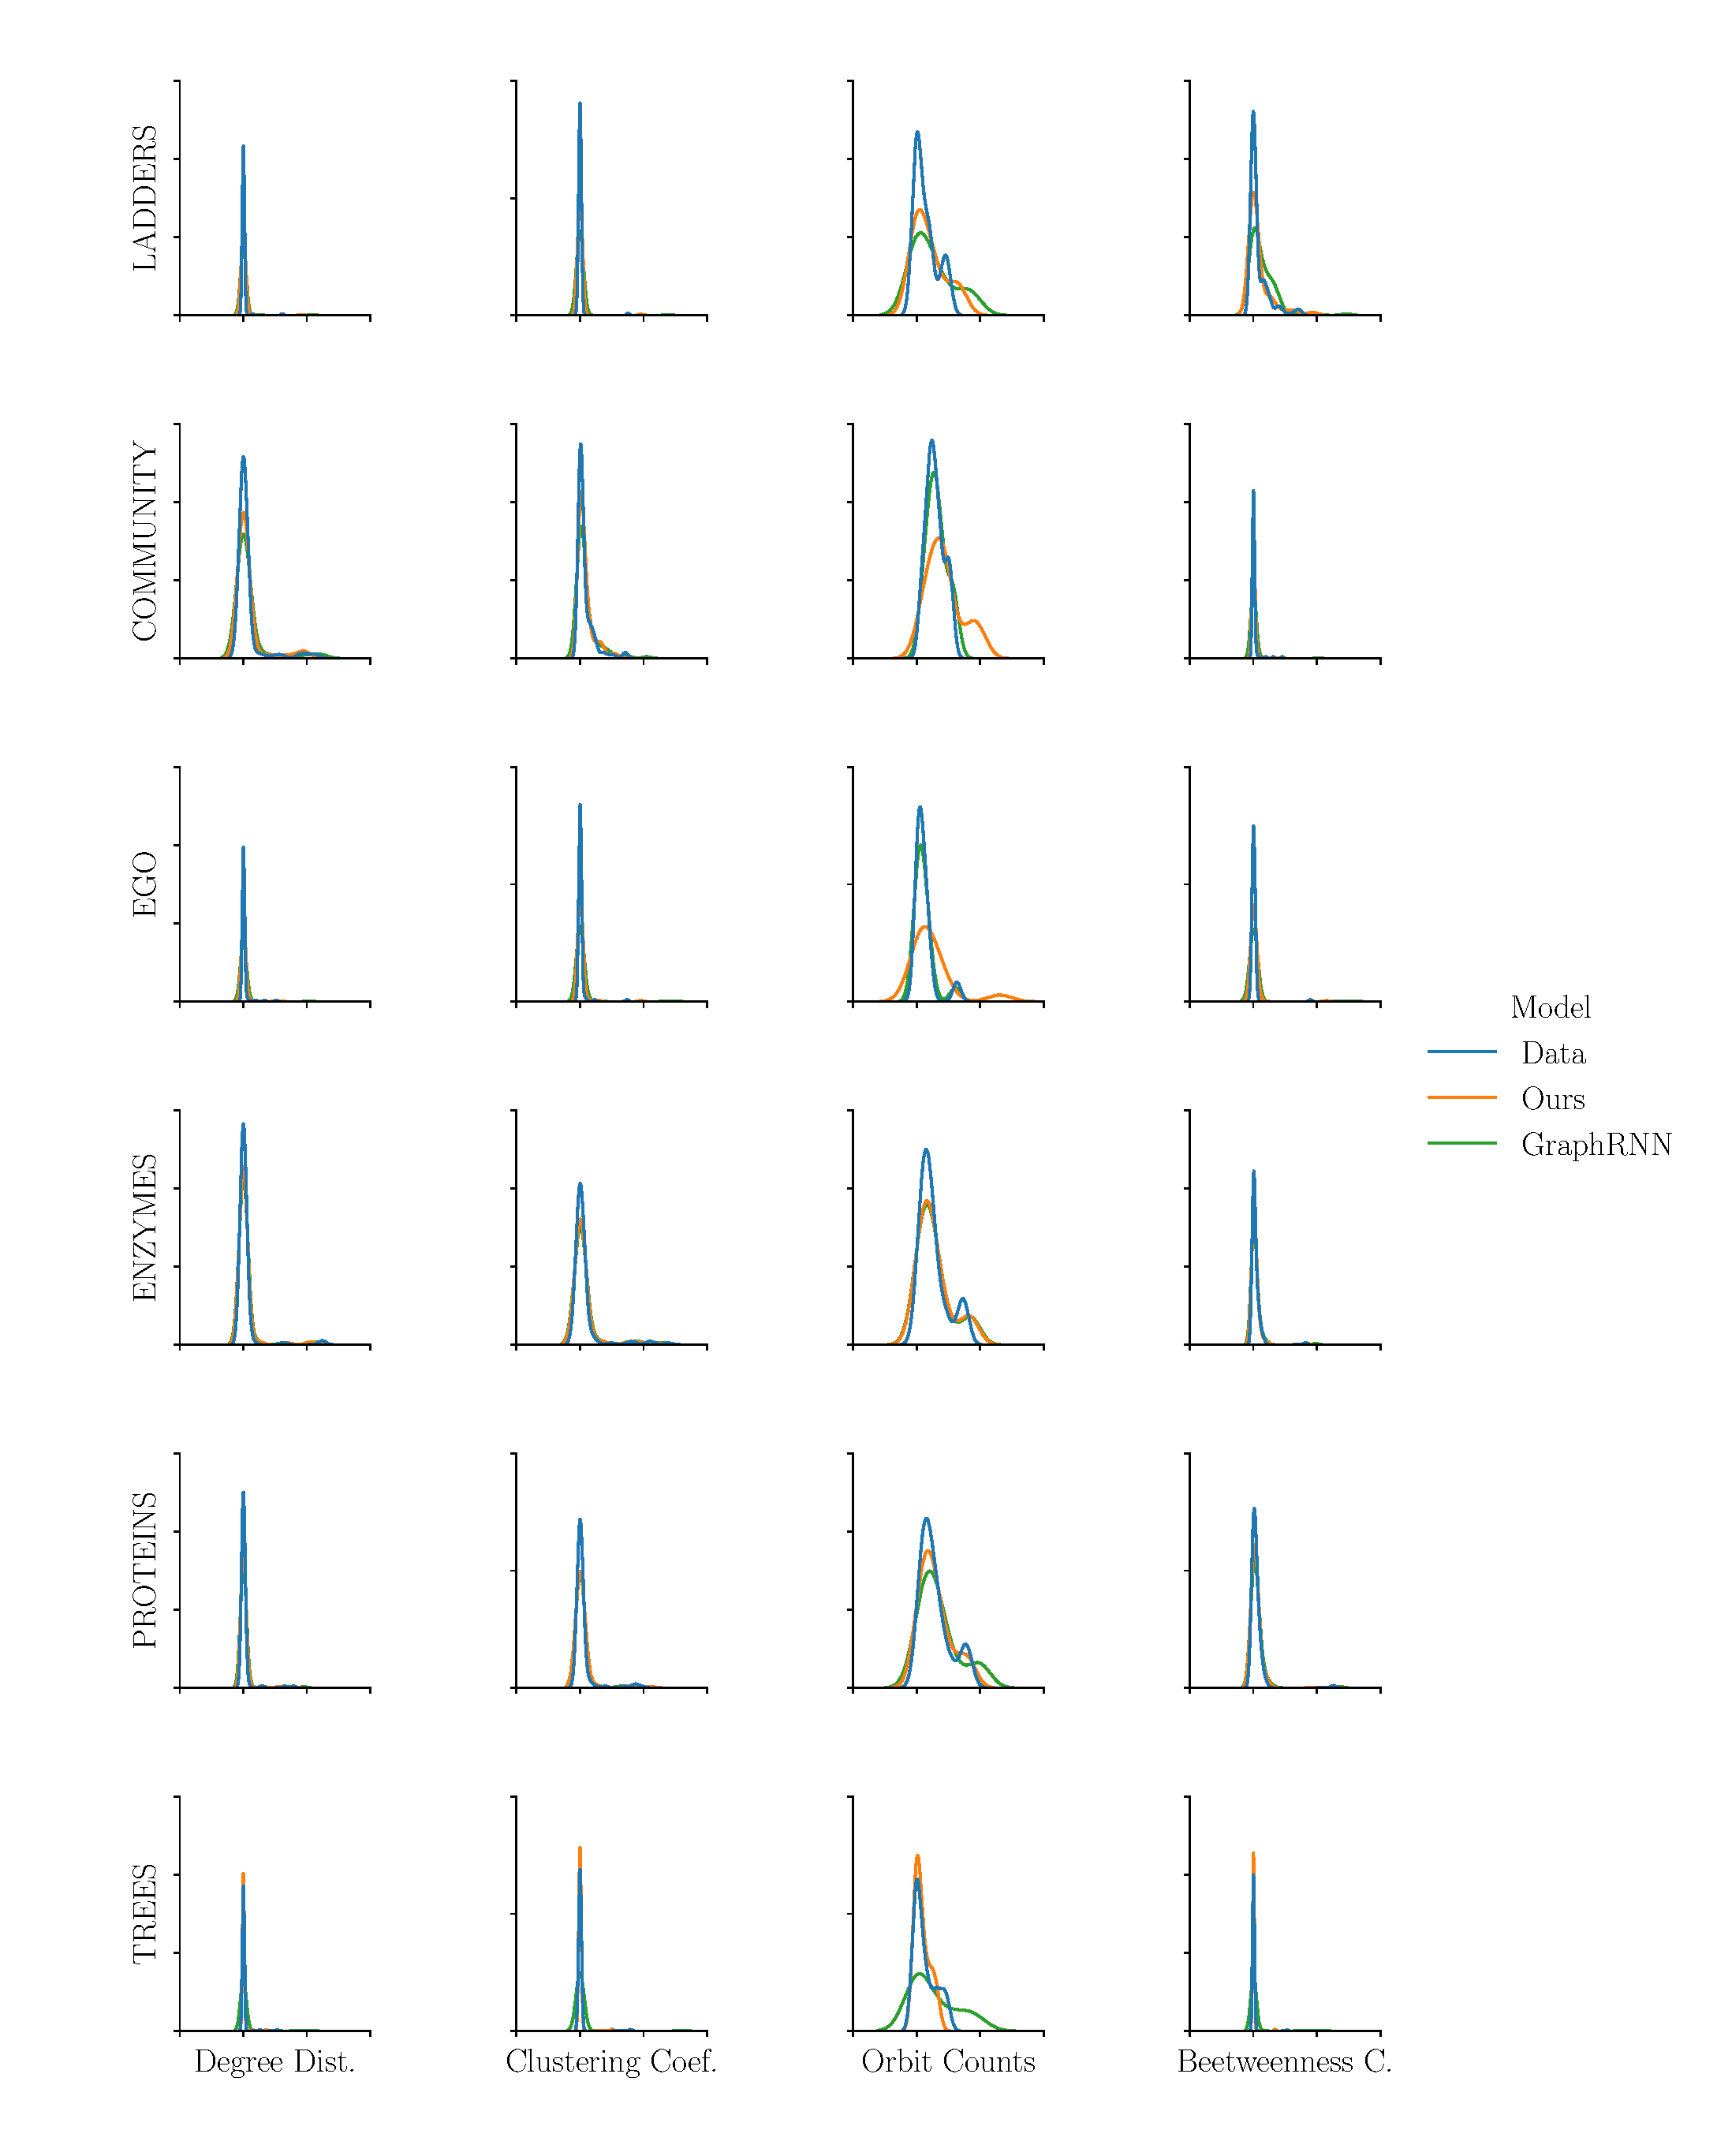
\includegraphics[width=\textwidth]{Figures/Chapter6/displot.eps}
\caption{We plot the KDE fitted on the histograms of graph statistics, taken both from the test and generated samples. Scales are omitted since values are normalized.}
\label{fig:distributions}
\end{figure}
Finally, in Figure \ref{fig:samples} we show graphs drawn from our model against real graphs, on three datasets. Indeed, visual inspection confirms that generated graphs display connectivity patterns typical of real graphs, for example ego nodes in EGO-like graphs, long chains in PROTEINS-like graphs, and dense clusters in  COMMUNITY-like graphs.
\begin{figure}[h!]
\centering
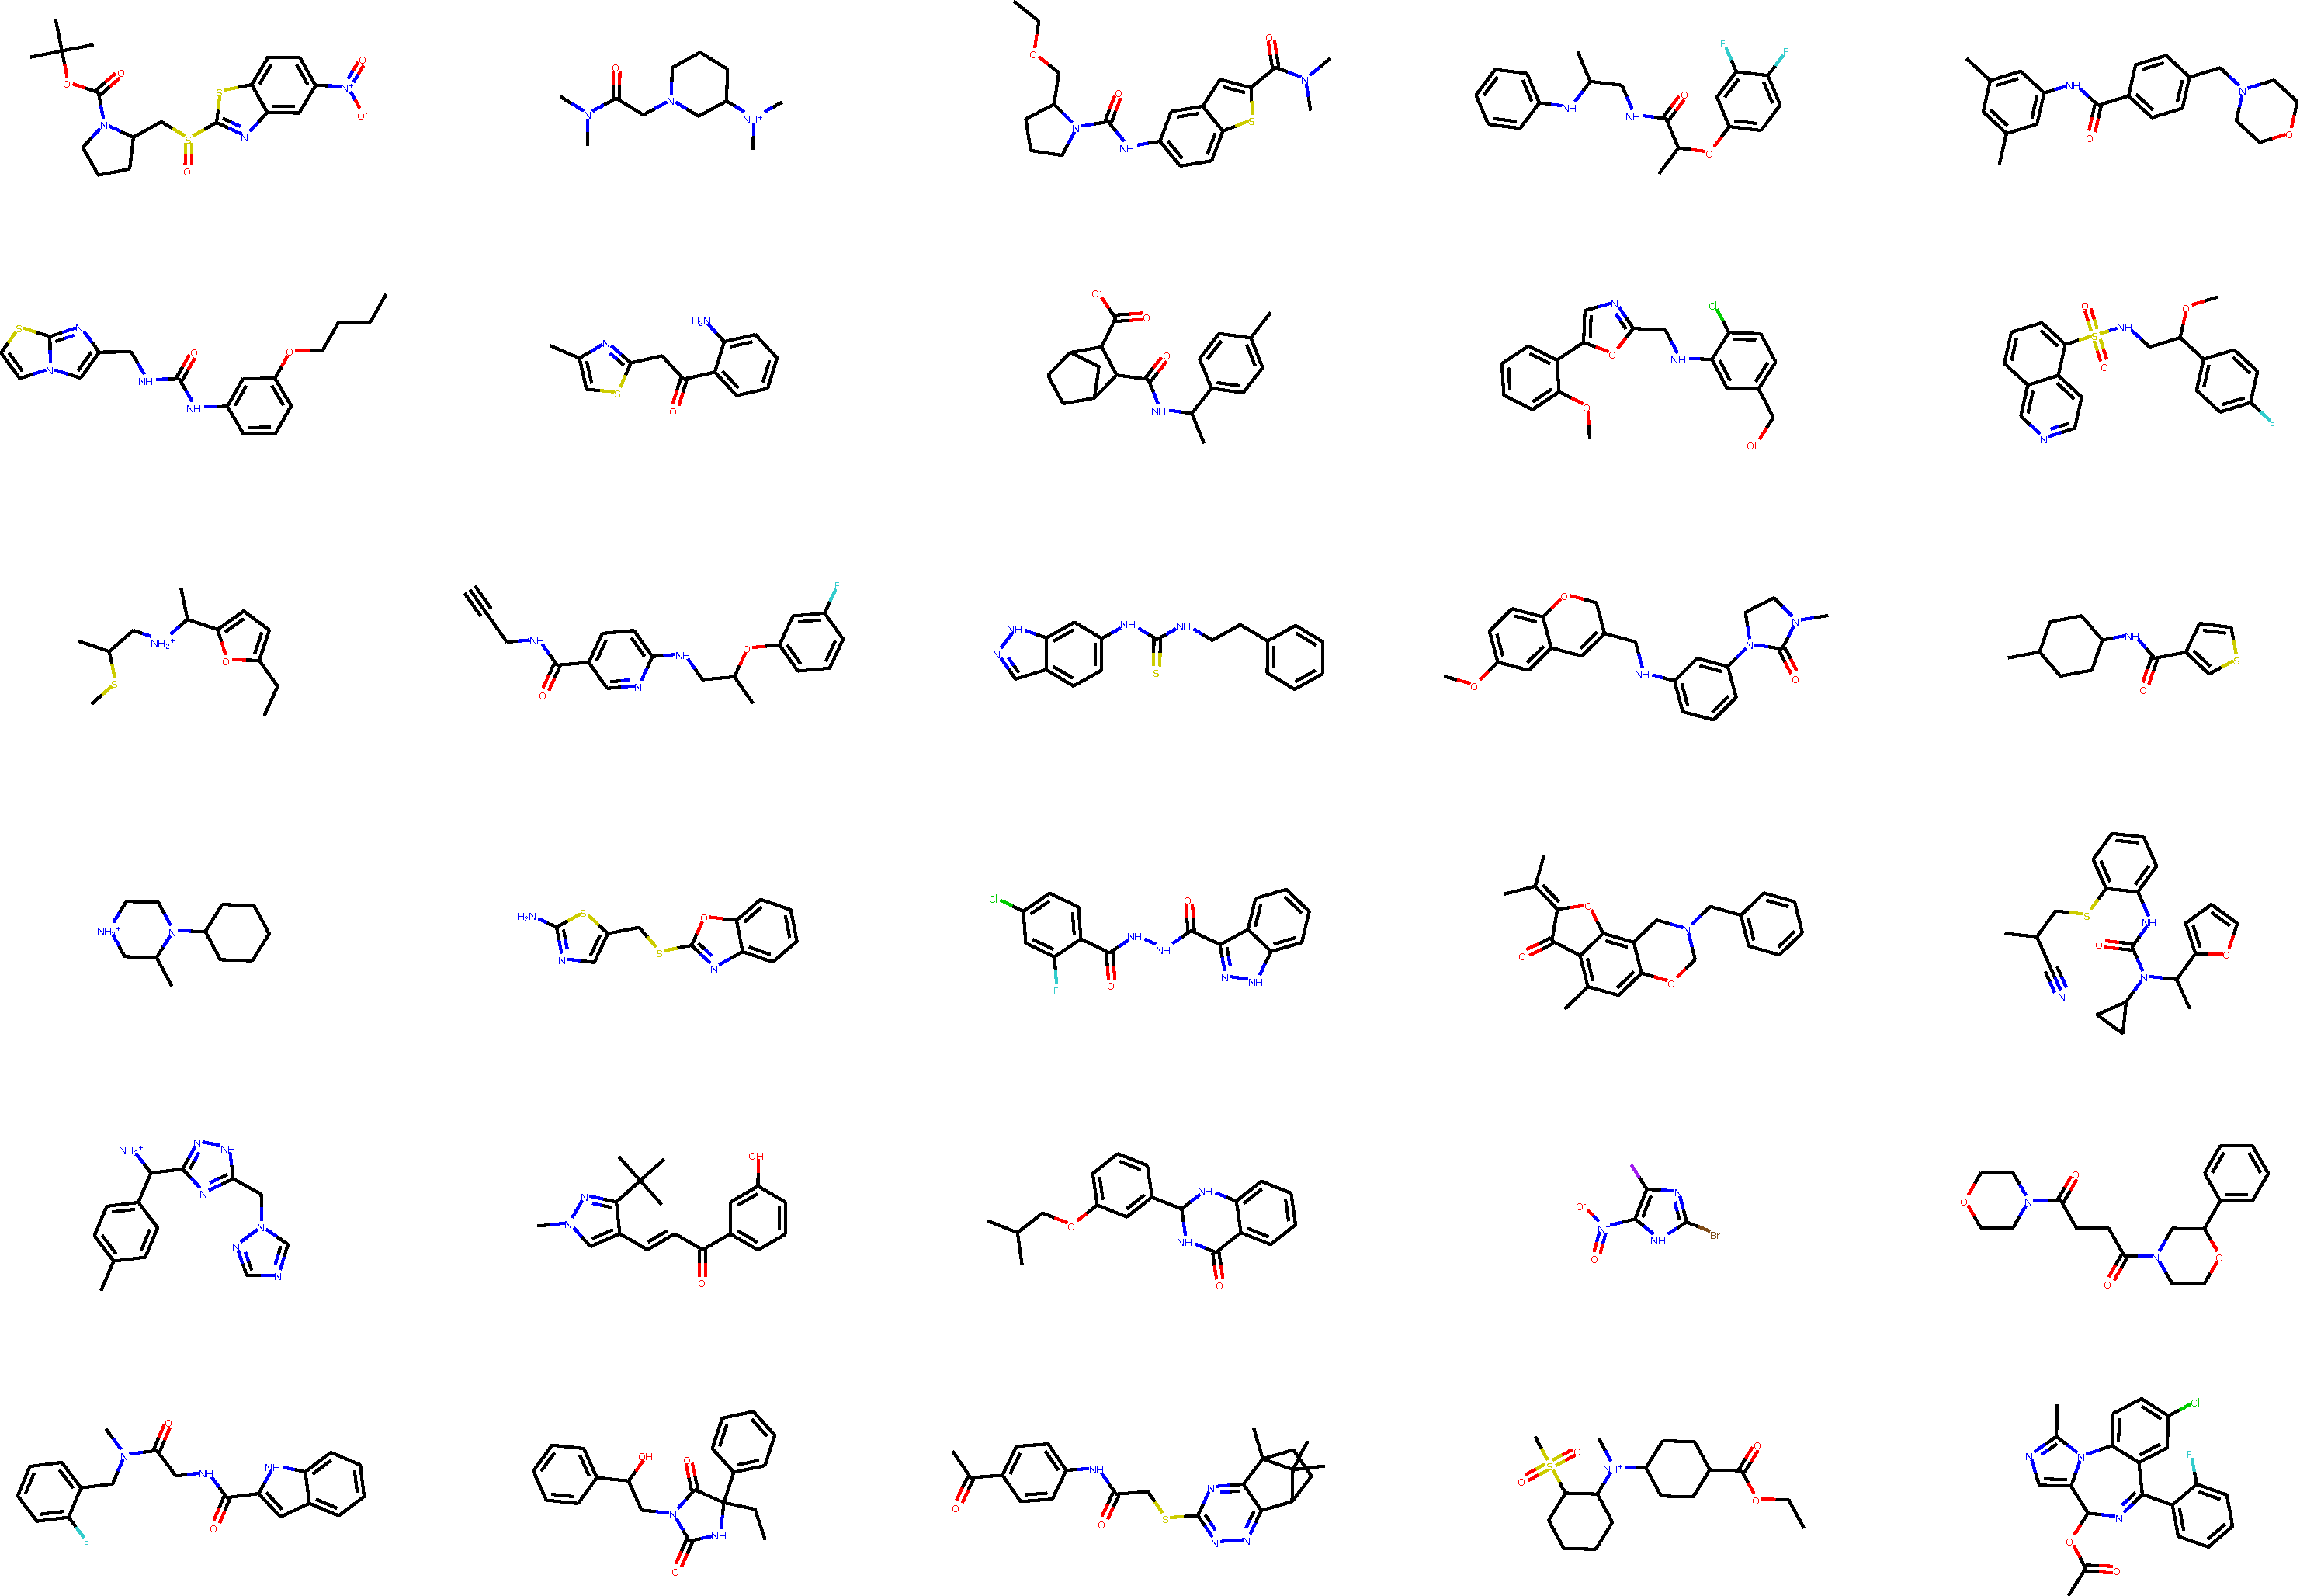
\includegraphics[width=\textwidth]{Figures/Chapter6/samples.eps}
\caption{Five randomly chosen graphs, both from the training sample (left) and generated by our model (right), on each considered dataset (displayed by row). Notice how our generative model has picked up all the characterizing connectivity patterns.}
\label{fig:samples}
\end{figure}

\subsection{Effect of Node Ordering}
In a follow-up study, we investigate if the way nodes are ordered during the graph preprocessing phase affects performances. To do so, we compare the proposed model with ablated models, where graphs are transformed into ordered edge sequences using different node orderings. Specifically, we focus on five different ablations:
\begin{itemize}
    \item \emph{Random}: the ordered edge sequence is constructed with a random permutation of the nodes. This strategy is expected to perform very poorly, since the model does not \quotes{see} consistent connectivity patterns during training;
    \item \emph{BFS Random}: the ordered edge sequence is constructed using the strategy proposed by \citet{you2018graphrnn}; that is, the ordered edge sequence is constructed using the BFS order, but each time a graph is picked from the training set at different epochs, the root node for the visit can be different. The strategy corresponds to train the model on every possible node permutation induced by a breadth-first search (BFS) visit of the graph. On one hand, this strategy acts as a regularizer, since at each epoch the training set changes completely. On the other hand, however, changing the node ordering at each epoch could in principle prevent our model from focusing on useful connectivity patterns, simply because they are \quotes{masked} away by different node permutations;
    \item \emph{DFS Random}: the same strategy as BFS random, but using depth-first search (DFS) visit instead;
    \item \emph{DFS}: a strategy equivalent to the one proposed in this work, which uses depth-first traversal instead of breadth-first;
    \item \emph{SMILES}: for the two molecular datasets only, the node ordering imposed by the SMILES linearization of the graph.
\end{itemize}
The ablation experiment consists of training the models with the alternative node ordering strategies for 1000 epochs without regularization. In practice, we try to overfit the dataset on purpose. The idea is to assess whether the alternative node ordering strategies are able to memorize connectivity patterns (hence, given proper regularization, are able to generalize to unseen ones). As a further experiment, we perform a qualitative evaluation similarly to Section \ref{sec:qualitative-analysis}.

In Figure \ref{fig:loss}, we plot the loss obtained by the different ablations across all the datasets. The figure shows that the models trained with the BFS, DFS and SMILES ordering strategies are able to reach a lower loss than the random ablations, which in contrast plateau at higher loss values. This experiment supports the choice of the BFS node ordering, which couples well with the architecture of our model, and provides an effective inductive bias to learn connectivity patterns from very different graph datasets.

\begin{figure}[h!]
\centering
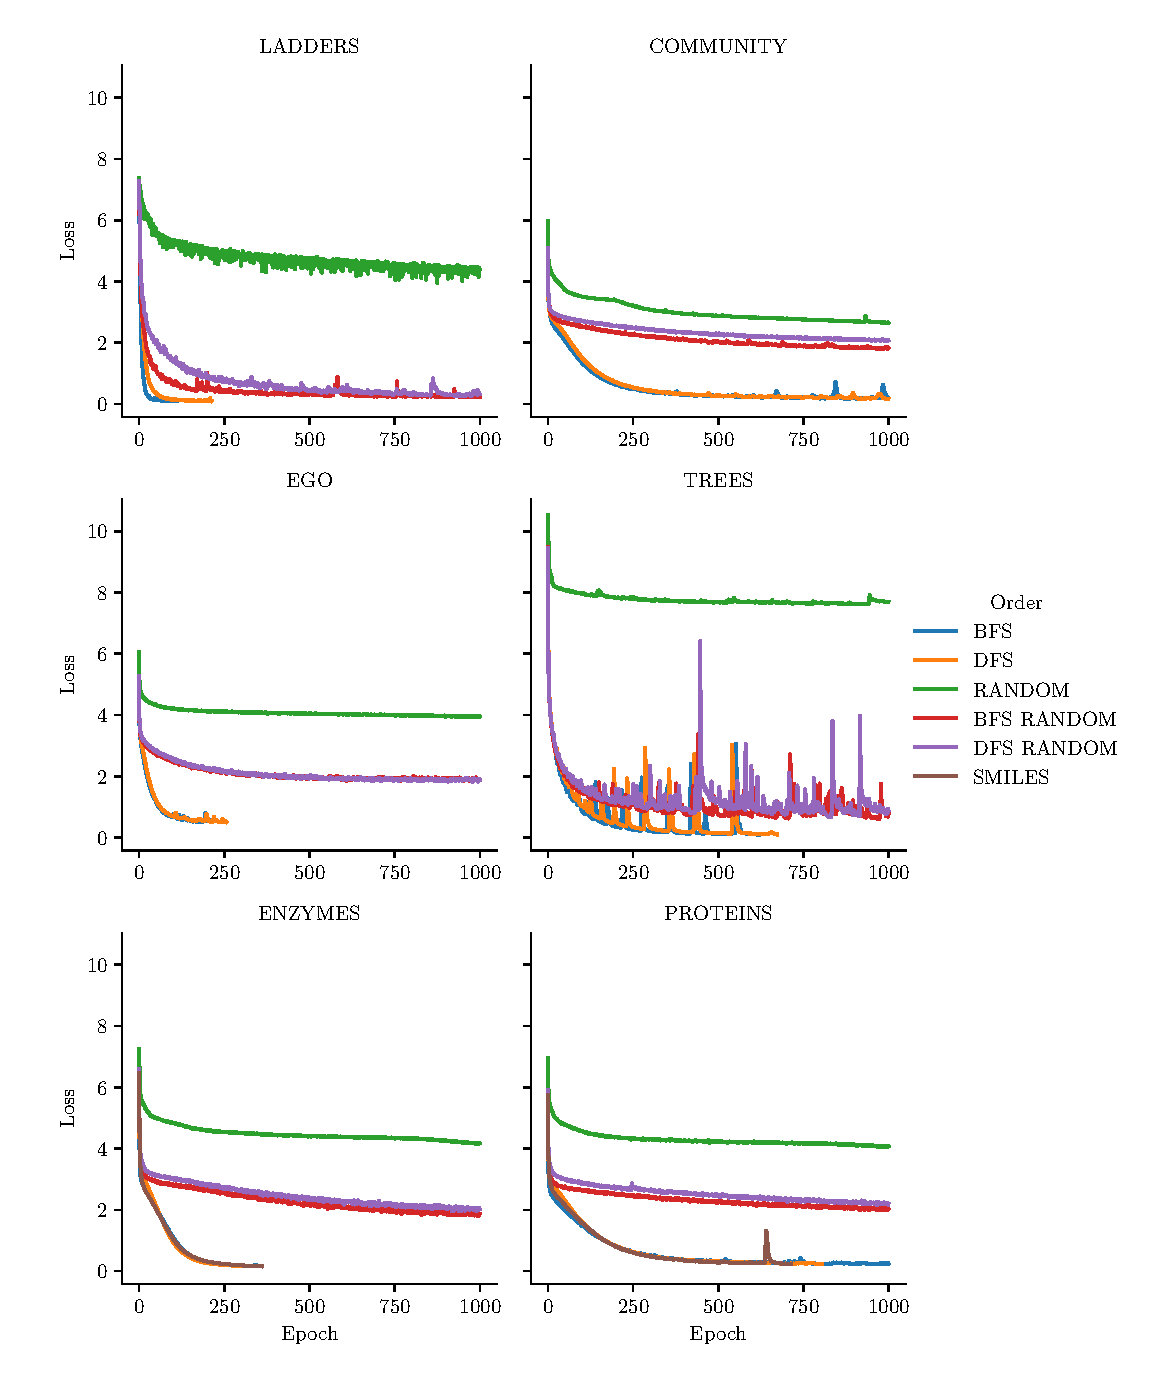
\includegraphics[width=\textwidth]{Figures/Chapter6/loss.eps}
\caption{Plot of the loss on dataset Protein of variants of our approach trained under different node orderings. Notice how the models trained with our proposed node ordering (blue), and SMILES (orange) are able to reach a lower training loss in a smaller number of epochs, compared to variants trained with random ordering (red) and BFS random ordering (green).}
\label{fig:loss}
\end{figure}
The results of the qualitative analysis are detailed in Table \ref{tab:graph-ordering-qualitative}. It can be easily noticed that the proposed node ordering strategy yields superior results in every chosen metric, compared to the ablations. The only competitive node ordering strategy is DFS, which basically differs from ours in the way graph nodes are visited. However, despite its similarity to our choice, this strategy seems to underperform in some cases, for example in all the local metrics in the COMMUNITY dataset. To explain this phenomenon, we hypothesize that the choice of DFS traversal instead of BFS is less suited to capture local dependencies. In conclusion, these results further extend the evidences supporting the robustness of our approach.

\begin{table}
    \footnotesize
    \centering
    \caption{We show the results of training the model with different node ordering strategies. Best performances are bolded.}
    \label{tab:graph-ordering-qualitative}
    \begin{tabular}{lccccccc}
        \toprule
        \textbf{Dataset} & \textbf{Metric} & \textbf{Random} & \textbf{Rand. BFS} & \textbf{Rand. DFS} & \textbf{DFS} & \textbf{SMILES} & \textbf{Ours}\\
        \midrule
          & DD             & 0.881 (0.111) & 0.162 (0.010) & 0.079 (0.011) & 0.073 (0.012) & - & \textbf{0.013} (0.003)\\
          & CC             & 0.317 (0.019) & 0.025 (0.006) & 0.015 (0.007) & 0.002 (0.003) & - & \textbf{0.000} (0.000)\\
LADDERS   & OC             & 0.136 (0.015) & 0.007 (0.001) & 0.003 (0.001) & 0.002 (0.001) & - & \textbf{0.000} (0.000)\\
          & BC             & 1.111 (0.080) & 0.411 (0.053) & 0.283 (0.070) & \textbf{0.202} (0.018) & - & 0.762 (0.180)\\
          & NSPDK          & 0.549 (0.006) & 0.230 (0.032) & 0.089 (0.018) & 0.114 (0.016) & - & \textbf{0.056} (0.022)\\
        \midrule
          & DD             & 0.204 (0.002) & 0.027 (0.001) & 0.073 (0.004) & 0.025 (0.002) & - & \textbf{0.013} (0.000)\\
          & CC             & 11.066 (0.990) & 2.858 (0.340) & 0.368 (0.025) & 0.471 (0.022) & - & \textbf{0.101} (0.011)\\
COMMUNITY & OC             & 1.142 (0.020) & 0.276 (0.002) & 0.045 (0.002) & 0.088 (0.002) & - & \textbf{0.013} (0.002)\\
          & BC             & 0.876 (0.132) & 1.229 (0.012) & 0.232 (0.046) & 0.177 (0.045) & - & \textbf{0.038} (0.005)\\
          & NSPDK          & 0.062 (0.001) & 0.031 (0.000) & 0.024 (0.001) & 0.012 (0.001) & - & \textbf{0.009} (0.000)\\
        \midrule
          & DD             & 0.099 (0.002) & 0.039 (0.004) & 0.052 (0.002) & \textbf{0.026} (0.002) & - & \textbf{0.029} (0.001)\\
          & CC             & 0.241 (0.004) & 0.301 (0.002) & 0.233 (0.002) & \textbf{0.073} (0.007) & - & \textbf{0.090} (0.011)\\
EGO       & OC             & 0.109 (0.002) & 0.055 (0.002) & 0.039 (0.000) & \textbf{0.004} (0.001) & - & \textbf{0.002} (0.001)\\
          & BC             & 0.139 (0.012) & 0.141 (0.001) & 0.139 (0.001) & \textbf{0.052} (0.013) & - & 0.096 (0.001)\\
          & NSPDK          & 0.010 (0.000) & 0.011 (0.001) & 0.018 (0.000) & \textbf{0.007} (0.000) & - & 0.016 (0.001)\\
        \midrule
          & DD             & 0.819 (0.004) & 0.320 (0.010) & 0.261 (0.007) & 0.143 (0.008) & - & \textbf{0.078} (0.002)\\
          & CC             & 0.065 (0.001) & 0.004 (0.001) & 0.003 (0.000) & 0.004 (0.001) & - & \textbf{0.000} (0.000)\\
TREES     & OC             & 0.028 (0.001) & 0.005 (0.001) & 0.004 (0.000) & 0.003 (0.000) & - & \textbf{0.001} (0.000)\\
          & BC             & 0.416 (0.008) & 0.075 (0.002) & 0.067 (0.002) & \textbf{0.056} (0.003) & - & \textbf{0.056} (0.008)\\
          & NSPDK          & 0.653 (0.003) & 0.328 (0.004) & 0.240 (0.005) & 0.142 (0.009) & - & \textbf{0.042} (0.004)\\
        \midrule
          & DD             & 0.499 (0.014) & 0.140 (0.005) & 0.135 (0.007) & 0.064 (0.004) & 0.077 (0.007) & \textbf{0.040} (0.002)\\
          & CC             & 0.581 (0.026) & 1.107 (0.218) & 0.566 (0.032) & 0.138 (0.009) & 0.230 (0.011) & \textbf{0.128} (0.037)\\
ENZYMES   & OC             & 0.096 (0.002) & 0.179 (0.007) & 0.102 (0.001) & 0.019 (0.003) & 0.034 (0.003) & \textbf{0.005} (0.002)\\
          & BC             & 2.484 (0.038) & 1.192 (0.022) & 0.293 (0.029) & 0.138 (0.005) & 0.479 (0.088) & \textbf{0.062} (0.006)\\
          & NSPDK          & 0.113 (0.002) & 0.045 (0.000) & 0.041 (0.001) & 0.026 (0.001) & 0.030 (0.002) & \textbf{0.021} (0.001)\\
        \midrule
          & DD             & 0.209 (0.007) & 0.160 (0.002) & 0.153 (0.008) & 0.092 (0.006) & 0.104 (0.008) & \textbf{0.018} (0.003)\\
          & CC             & 0.947 (0.025) & 1.105 (0.019) & 0.568 (0.034) & 0.163 (0.003) & 0.277 (0.007) & \textbf{0.056} (0.005)\\
PROTEINS  & OC             & 0.200 (0.006) & 0.220 (0.001) & 0.120 (0.003) & 0.032 (0.003) & 0.067 (0.006) & \textbf{0.002} (0.000)\\
          & BC             & 1.161 (0.144) & 0.345 (0.015) & 0.157 (0.019) & 0.071 (0.003) & 0.368 (0.124) & \textbf{0.048} (0.005)\\
          & NSPDK          & 0.059 (0.001) & 0.045 (0.001) & 0.038 (0.001) & 0.026 (0.001) & 0.032 (0.002) & \textbf{0.017} (0.000)\\
        \bottomrule
    \end{tabular}
\end{table}